\documentclass[a4paper,onecolumn,10pt]{article}

\usepackage{polski}
\usepackage[utf8]{inputenc}
\usepackage{tgtermes}
\usepackage{tgcursor}
\usepackage[QX]{fontenc}
\usepackage[T1]{fontenc}
\usepackage{fancyhdr}
\usepackage{fancyvrb}
\usepackage{epsfig}
\usepackage{color}
\usepackage{listings} 
\usepackage{multicol}
\usepackage{capt-of}
\usepackage{url}
\usepackage{epstopdf}
\usepackage{tabularx}
\usepackage{enumitem}

% % % % % % % % % zwiększenie możliwości zagnieżdżenia wyliczeń : http://tex.stackexchange.com/questions/41408/a-five-level-deep-list
\setlistdepth{7}

\newlist{myEnumerate}{enumerate}{7}
\setlist[myEnumerate,1]{label*=\arabic*.}
\setlist[myEnumerate,2]{label*=\arabic*.}
\setlist[myEnumerate,3]{label*=\arabic*.}
\setlist[myEnumerate,4]{label*=\arabic*.}
\setlist[myEnumerate,5]{label*=\arabic*.}
\setlist[myEnumerate,6]{label*=\arabic*.}
\setlist[myEnumerate,7]{label*=\arabic*.}
% % % % % % % % % % % % % % % % % % % % % % % % % % % % % % % % %
%% Two counters to keep track of categories and 
%% subcategories

\usepackage{listings}
\usepackage{color}
\usepackage{lastpage}

\setlength{\headheight}{12.02503pt}

\usepackage{hyperref}
\usepackage{fancyhdr}

\begin{document}
\pagestyle{fancy}
\lhead{Moduł rejestru dostępnych zasobów}
\chead{}
\rhead{APSI}
\lfoot{Dokumentacja projektowa}
\cfoot{wersja 0.1}
\rfoot{\thepage\ / \pageref{LastPage}}
\renewcommand{\headrulewidth}{0.4pt}
\renewcommand{\footrulewidth}{0.4pt}

\title{
\begin{huge}
	\textit{\textbf{Moduł rejestru dostępnych zasobów}}
\end{huge}
\begin{small}
	\\ Dokumentacja projektowa \vspace{135mm}
\end{small}}

\author{
\begin{tabular}{l l}	
		Zespół \textbf{A07/14Z}: & \\ \\ 
		Dziurdziak Mateusz &  Niedźwiedź Andrzej  \\ 
 	Gadawski Łukasz &  	Opasiak Krzysztof  \\ 
 	Marcinkowski Łukasz & \\ \\ \\  
\end{tabular}
}

\maketitle
\thispagestyle{empty}
\tableofcontents

%\chapter{pierwsz}
\section{Wstęp}

% Wszelkie podobieństwo do realnych firm a tym bardziej fikcyjnych jest przypadkowe :D:D:D
Duża firma informatyczna {\bf Nabiano} ze względu na swój dynamiczny
rozwój zleciła opracowanie zintegrowanego systemu wspomagającego
zarządzanie pracownikami oraz wszelkimi zasobami wykorzystywanymi w
firmie.

Ponieważ powstający system jest bardzo rozbudowany, główny wykonawca
postanowił zastosować w nim architekturę modularną. W skład systemu
wchodzą następujące moduły:

\begin{itemize}
\item[--] moduł repozytorium dokumentów wraz z mechanizmem obiegu dokumentów,
\item[--] moduł rejestru pracowników i wykonywanych prac,
\item[--] moduł rejestru dostępnych zasobów,
\item[--] moduł alokacji zasobów i planowania obsady projektów,
\item[--] moduł repozytorium wymagań dla projektów,
\item[--] moduł repozytorium testów,
\item[--] moduł repozytorium problemów technicznych.
\end{itemize}

Projekt oraz implementacja poszczególnych modułów została przekazana
podwykonawcom. Jednym z nich jest firma {\bf ELKA-Infor}. Jest ona
odpowiedzialna za przygotowanie projektu modułu rejestru dostępnych
zasobów oraz jego implementację.

Niniejszy dokument został przygotowany przez podwykonawce (ELKA-Infor)
jako dokumentacja projektowa do tworzonego modułu rejestru dostępnych
zasobów. Dokument ten ma na celu ułatwić współprace z głównym
wykonawcą, a także pozwolić na specyfikację wymagań wobec innych
modułów wchodzących w skład systemu.

\subsection{Opis działalności}

Firma Nabiano działa na polskim rynku od dziesięciu lat. Została ona
założona przez jej obecnego prezesa Pana Siergija Wybora. We wczesnej
fazie rozwoju firma zajmowała się sprzedażą sprzętu komputerowego
oraz oprogramowania w kilku punktach w Białymstoku. W roku 2007 firma
rozszerzyła znacząco zakres swojej działalności i ukierunkowała się na
klienta biznesowego poprzez wprowadzenie do swojej oferty sprzętu
serwerowego oraz oprogramowania CMS firmy Atlasin.

Znaczący wzrost liczby zatrudnionych pracowników miał miejsce w 2009
roku, kiedy to firma postanowiła zainwestować duże środku i przy
wsparciu funduszy unijnych otworzyła dział rozwojowy w Łodzi, którego celem
było stworzenie własnego systemu CMS. Pierwsza wersja systemu powstała
już w 2010 roku i zakupiło ją kilka firm oraz jedna z największych w
Polsce korporacji.

Kolejnym krokiem milowym w rozwoju firmy było podpisanie w 2012 roku
kontraktu z rządem Korei Północnej na dostarczenie elektronicznego
systemu wyborczego na wybory parlamentarne w 2014. Projekt ten
stanowił dla firmy ogromne wyróżnienie oraz wyzwanie. Aby podołać temu
trudnemu zleceniu zwiększono zatrudnienie do ponad 1000 pracowników
oraz otwarto nowe oddziały w Warszawie oraz Pjongjang. W styczniu 2014
roku pomyślnie wdrożono wspomniany wcześniej system wyborczy. W marcu
tego samego roku odbyły się przy użyciu tego systemu wybory
parlamentarne. System działał bez żadnych zakłóceń oraz awarii. Po
wygranych przez {\it Kim Dzong Una} wyborach parlamentarnych firma
otrzymała list gratulacyjny oraz obietnicę polecenia tego systemu
wyborczego przywódcą innych państw. Już po pół roku od udanego
wdrożenia systemu wyborczego w Korei do firmy zaczęły napływać
zamówienia z całego świata, między innymi z Białorusi, Kuby oraz
Rosji. Swoje zainteresowanie wyraziły również inne państwa
europejskie, które mają problemy ze swoimi systemami wyborczymi.

W chwili obecnej firma Nabiano ponownie zwiększa swoje zatrudnienie i
rozpoczyna realizację kolejnych projektów. Na początku 2015 roku
planowane jest otwarcie oddziału firmy w Moskwie, a w 2016 roku w
Mińsku. Ze względu na ten dynamiczny rozwój firma postanowiła wdrożyć
system wspomagający zarządzania pracownikami, projektami oraz
wszystkimi środkami firmy.

\subsection{Przeznaczenie systemu}

W chwili obecnej w posiadaniu firmy znajduje się:

\begin{itemize}
\item[--] około 50 pojazdów
\item[--] około 800 telefonów
\item[--] około 1500 komputerów stacjonarnych
\item[--] około 2500 monitorów komputerowych
\item[--] około 2000 laptopów
\item[--] około 100 serwerów
\item[--] około 200 sztuk sprzętu serwerowego
\item[--] około 10000 sztuk innego drobnego sprzętu komputerowego
\item[--] około 300 nośników z oprogramowaniem
\item[--] około 200 licencji na użytkowanie oprogramowania (jedna licencja na wiele stanowisk)
\end{itemize}

Zarządzanie tymi zasobami w chwili obecnej wymaga znacznego wkładu
pracowników. Firma zatrudnia obecne około 40 pracowników, którzy
zajmują się zarządzaniem jej środkami. Wśród tych pracowników znajduje
się również grupa odpowiedzialna za komunikację z zewnętrznymi firmami
serwisującymi posiadane urządzenia. Pracownicy Ci rozlokowani są w
różnych oddziałach firmy więc ich podstawowym problemem jest brak
możliwości bezpośredniej komunikacji i współpracy.

Bieżący system zarządzania środkami oparty jest o setki arkuszy
kalkulacyjnych trzymanych na wewnętrznym serwisie firmowym. Taki
sposób pracy bardzo utrudnia śledzenie zarówno bieżącego stanu
sprzętowego (utrudniona agregacja) oraz powiązanie pomiędzy problemami
zgłaszanymi przez pracowników, a zleceniami serwisowania
sprzętu. Istotnym problemem jest również śledzenie zmian obecnych
użytkowników sprzętu, a także historii jego przekazywania pomiędzy
pracownikami.

Ze względu na wspomniane problemu firma postanowiła przy wdrożeniu
nowego systemu wspierającego jej funkcjonowanie utworzyć również moduł
zarządzania zasobami opisany w tym dokumencie. Moduł ten ma rozwiązać
wszystkie problemy obecne w obecnym systemie. W celu umożliwienia
prawidłowego funkcjonowania całego systemu moduł ten musi
współpracować z modułem pracowników w zakresie własności oraz
bieżącego użytkowania oraz z repozytorium problemów w celu śledzenia
problemów zgłaszanych przez użytkowników oraz śledzenia realizacji
zleceń serwisowych.


\section{Analiza wymagań}

\subsection{Wymagania funkcjonalne}

\begin{myEnumerate}
\item \textbf{Zarządzanie zasobami.}
	\begin{myEnumerate}
	\item Przeszukiwanie zasobów.
	\item Katalogowanie zasobów.
	\begin{myEnumerate}
	\item Obsługa sprzętu komputerowego.
	\begin{myEnumerate}
		\item Dodanie zasobu.
		\begin{myEnumerate}
		\item Dodanie podstawowych informacji o zasobie.
		\item Dodanie informacji o elementach wchodzących w skład zasobu.
		\item Zapisanie konfiguracji sprzętu komputerowego.
		\end{myEnumerate}
		\end{myEnumerate}
		\item Edycja informacji o zasobie.
		\item Usunięcie zasobu z systemu.
	\end{myEnumerate}
	\item Obsługa oprogramowania.
	\begin{myEnumerate}
		\item Dodanie zasobu.
		\begin{myEnumerate}
			\item Dodanie podstawowych informacji o zasobie.
			\item Dodanie informacji o instalacji oprogramowania.
		\end{myEnumerate}
		\item Edycja informacji o zasobie.
		\item Usunięcie zasobu z systemu.
	\end{myEnumerate}
	\item Obsługa innego sprzętu, urządzeń i wyposażenia.
	\begin{myEnumerate}
		\item Dodanie zasobu.
		\begin{myEnumerate}
			\item Dodanie podstawowych informacji o zasobie.
		\end{myEnumerate}
		\item Edycja informacji o zasobie.
		\item Usunięcie zasobu z systemu.
	\end{myEnumerate}
	\item Obsługa czasopism oraz literatury.
	\begin{myEnumerate}
		\item Dodanie zasobu.
		\begin{myEnumerate}
			\item Dodanie podstawowych informacji o zasobie.
		\end{myEnumerate}
		\item Edycja informacji o zasobie.
		\item Usunięcie zasobu z systemu.
	\end{myEnumerate}
	\item Współpraca z modułem rejestru pracowników.
	\begin{myEnumerate}
	\item Zapisanie informacji o osobie odpowiedzialnej za dany zasób.
	\item Zapisanie informacji o użytkowniku konkretnego zasobu.
	\end{myEnumerate}
	\item Obliczanie statystyk.
	\begin{myEnumerate}
	\item Prezentacja zakupów konkretnych zasobów w poszczególnych latach.
	\item Prezentacja ilości zasobów w poszczególnych działach.
	\item Prezentacja ilość zasobów w poszczególnych placówkach.
	\end{myEnumerate}
	\end{myEnumerate}
\item \textbf{Zarządzanie serwisem sprzętu oraz oprogramowania.}
	\begin{myEnumerate}
		\item Rejestracja informacji dotyczącej miejsca zakupu.
		\item Historia napraw sprzętu.
			\begin{myEnumerate}
			\item Rejestracja informacji o wewnętrznej naprawie sprzętu.
			\item Rejestracja naprawy sprzętu przez serwis zewnętrzny.
			\end{myEnumerate}
		\item Historia obsługi oprogramowania.
		\begin{myEnumerate}
		\item Rejestracja aktualizacji oprogramowania.
		\item Rejestracja "naprawy" oprogramowania.
		\end{myEnumerate}
		\item Współpraca z repozytorium problemów.
		\begin{myEnumerate}
		\item Rejestracja operacji serwisowej.
		\end{myEnumerate}
	\end{myEnumerate}
\end{myEnumerate}
\subsection{Wymagania niefunkcjonalne}
\subsection{Specyfikacja przypadków użycia - poziom ogólny}

\section{Architektura systemu}

\subsection{Dekompozycja..}
\subsection{Diagram1..}
\subsection{Diagram2..}

\section{Specyfikacja sprzętu}

\subsection{Schemat architektury}

\begin{figure}[H]
	\centering
	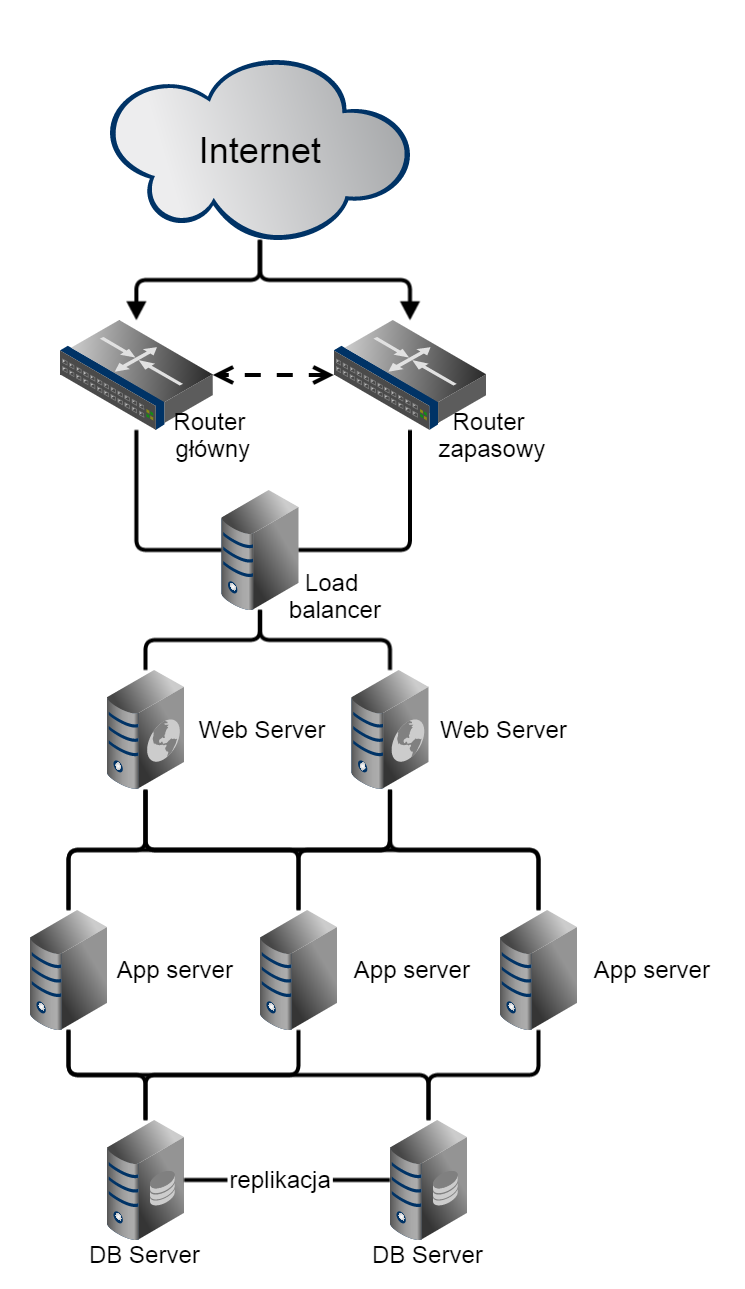
\includegraphics[height=0.8\textheight]{img/architektura}
	\caption{Schemat architektury \label{fig:labelArchitecture}}
\end{figure}


Jak uwidoczniono na \ref*{fig:labelArchitecture} na wejściu żądania będą obsługiwany przez router główny, któremu towarzyszył będzie router zapasowy w przypadku, kiedy router główny nie będzie w stanie obsłużyć żądania. Następnie wybierany będzie Web Server, który będzie obsługiwał zgłoszenie (w zależności od poziomu obciążenia serwerów, decydować o tym będzie Load Balancer). W analogiczny sposób wybierany będzie serwer aplikacyjny, pośredniczący w obsłudze.

W odniesieniu do serwerów bazy danych zastosowany będzie mechanizm replikacji danych, który ma zagwarantować bezpieczeństwo przechowywanych informacji (ochronę przed ich utratą w wyniku awarii jednego z serwerów).

\subsection{Oszacowanie rozmiarów systemu}

W chwili obecnej firma posiada w ewidencji:

\begin{itemize}
\item[--] około 50 pojazdów
\item[--] około 800 telefonów
\item[--] około 1500 komputerów stacjonarnych
\item[--] około 2500 monitorów komputerowych
\item[--] około 2000 laptopów
\item[--] około 100 serwerów
\item[--] około 200 sztuk sprzętu serwerowego
\item[--] około 10000 sztuk innego drobnego sprzętu komputerowego
\item[--] około 300 nośników z oprogramowaniem
\item[--] około 200 licencji na użytkowanie oprogramowania (jedna licencja na wiele stanowisk)
\end{itemize}

Oznacza to, że w ewidencji firmy jest ponad 17 tysięcy przedmiotów i
licencji na oprogramowanie. Ponieważ firma się intensywnie rozwija
należy założyć, że system będzie obsługiwał co najmniej 30 tysięcy
przedmiotów. W chwili obecnej firma zatrudnia około 1500
pracowników. Ponieważ firma przeżywa intensywny rozwój konieczne jest
zwymiarowanie systemu na poziomie co najmniej dwu krotności obecnego
zatrudnienia to jest 3000 pracowników. System należy do grupy systemów
wspierających funkcjonowanie przedsiębiorstwa i nie będzie
wykorzystywany w ramach podstawowych zadania pracowników. Należy zatem
założyć, że nie wszyscy pracownicy będą go używali w tym samym
czasie. W związku z tym należy założyć, że równocześnie system będzie
używany przez około 10\% pracowników czyli 300 osób. Powyższe szacunki
są zgodne z wymaganiami niefunkcjonalnymi przedstawionymi w
\ref{wymagania_niefunkcjonalne}.

\subsection{Rozkład obciążenia na poszczególne warstwy}

Aplikacja w architekturze trójwarstwowej posiada budowę bardzo
modularną, przez co możliwe jest rozmieszczenie różnych elementów na
odpowiednich maszynach. Dzięki takiemu rozmieszczeniu każda z warstw
może być wykonywana na sprzęcie dostosowanym do jej zadań. Ponieważ
każda warstwa wykonuje inne zadania to znacząco też różni się
charakterystyka sprzętu, który należy wykorzystać w danej warstwie.

\subsubsection{Warstwa prezentacji}

Warstwa prezentacji odpowiedzialna jest za wyświetlanie użytkownikowi
treści. Implementacja tej warstwy zostanie wykonana z użyciem języka
JavaScript wraz z technologiami HTML oraz CSS. Ponadto dodatkowa
funkcjonalność zostanie zaimplementowana przy użyciu biblioteki
jQuerry. Pomimo, iż zarówno serwer jak i klienci znajdować się będą w
sieci wewnętrznej przedsiębiorstwa należy zapewnić odpowiedni poziom
bezpieczeństwa poprzez wykorzystanie protokołu SSL/TLS.

Z perspektywy wymaganych zasobów sprzętowych wymagania dla tej warstwy
można podzielić na dwie części. Pierwsza z nich dotyczy wymagań co do
urządzenia na którym treść będzie prezentowana. Konieczne jest aby
takie urządzenie wyposażone było w przeglądarkę obsługującą
JavaScript. Druga część z wymagań sprzętowych dotyczy serwera www, do
którego kierowane będą żądania. Od tego urządzenia wymaga się przede
wszystkim wysokiej wydajności, krótkiego czasu odpowiedzi oraz
możliwości obsługi wielu klientów jednocześnie. Istotne jest również
zapewnienie wysokiej dostępności tego serwera.

\subsubsection{Warstwa logiki biznesowej}

Warstwa logiki biznesowej odpowiedzialna jest za przetwarzanie żądań
klienta w sposób zgodny z prawami rządzącymi organizacją. Zostanie ona
zaimplementowana w technologii J2EE. Jako serwer aplikacyjny wybrano
JBoos Application Server.

Z perspektywy wymaganych zasobów warstwa ta posiada analogiczne
wymagania jak warstwa prezentacji. Oznacza to, że istotna dostępność,
krótki czas odpowiedzi oraz możliwość obsługi wielu klientów
równocześnie. Te abstrakcyjne wymagania tej warstwy na sprzęt
przekładają się na duże zapotrzebowanie na procesor (w tym ich
liczbę), rozmiar pamięci RAM oraz szybkość odpowiedzi dysku twardego,
natomiast już sam rozmiar tego dysku może być nie zbyt duży.

\subsubsection{Warstwa danych}

Warstwa danych odpowiedzialna jest za przetwarzanie i przechowywanie
danych w sposób zapewniający ich spójność oraz trwałość. W tej
warstwie zostanie wykorzystana technologia Oracle DataBase 12c w
wersji Enterprise Edition. Jest to najnowsza wersja bazy danych od
Oracle i posiada wiele zaawansowanych mechanizmów, wpływających na
wydajność jak i bezpieczeństwo przechowywanych danych.

Z perspektywy wymaganych zasobów sprzętowych warstwa ta posiada
analogiczne wymagania co poprzednia lecz są one tutaj bardziej
krytyczne, gdyż zbyt długie przetwarzanie zapytania przez bazę danych
znacząco wydłuża czas odpowiedzi aplikacji. Należy również pamiętać o
dostosowaniu rozmiaru pamięci operacyjnej oraz zamontowaniu
odpowiedniej liczby wydajnych dysków twardych wraz z zapewnieniem ich
replikacji w celu zabezpieczenia się przed utrata danych.

\subsection{Sprzęt}

Budowa nowego systemu zarządzania przedmiotami i licencjami wymaga
znacznej rozbudowy dotychczasowej infrastruktury IT firmy.

\subsubsection{Warstwa prezentacji oraz aplikacji}

Część kliencka budowanego systemu będzie uruchamiana poprzez
przeglądarkę na komputerach pracowników firmy. Dzięki temu część
warstwy prezentacji, którą należy umieścić na serwerze składa się
wyłącznie z serwera WWW. Aby zatem ograniczyć konieczne zasoby
sprzętowe, a także opóźnienia w komunikacji pomiędzy warstwą
prezentacji, a warstwą aplikacji zdecydowano umieścić je na wspólnej
maszynie. Ponieważ klient ma wysokie wymagania co do dostępności
systemu, należy zakupić dwa serwery, które będą współdziałały i
dzieliły obciążenie pomiędzy siebie, a w razie awarii jednego z nich
drugi będzie w stanie zapewnić pełną funkcjonalność.


Jako serwer www oraz aplikacyjny powinna zostać wykorzystana maszyna,
która posiada wysoko wydajne procesory oraz pamięć RAM. Ważna jest
również możliwość montażu dysków twardych o krótkim czasie dostępu. W
związku z powyższym zdecydowano o wykorzystaniu serwerów Dell
PowerEdge R630.

\begin{figure}[H]
	\centering
	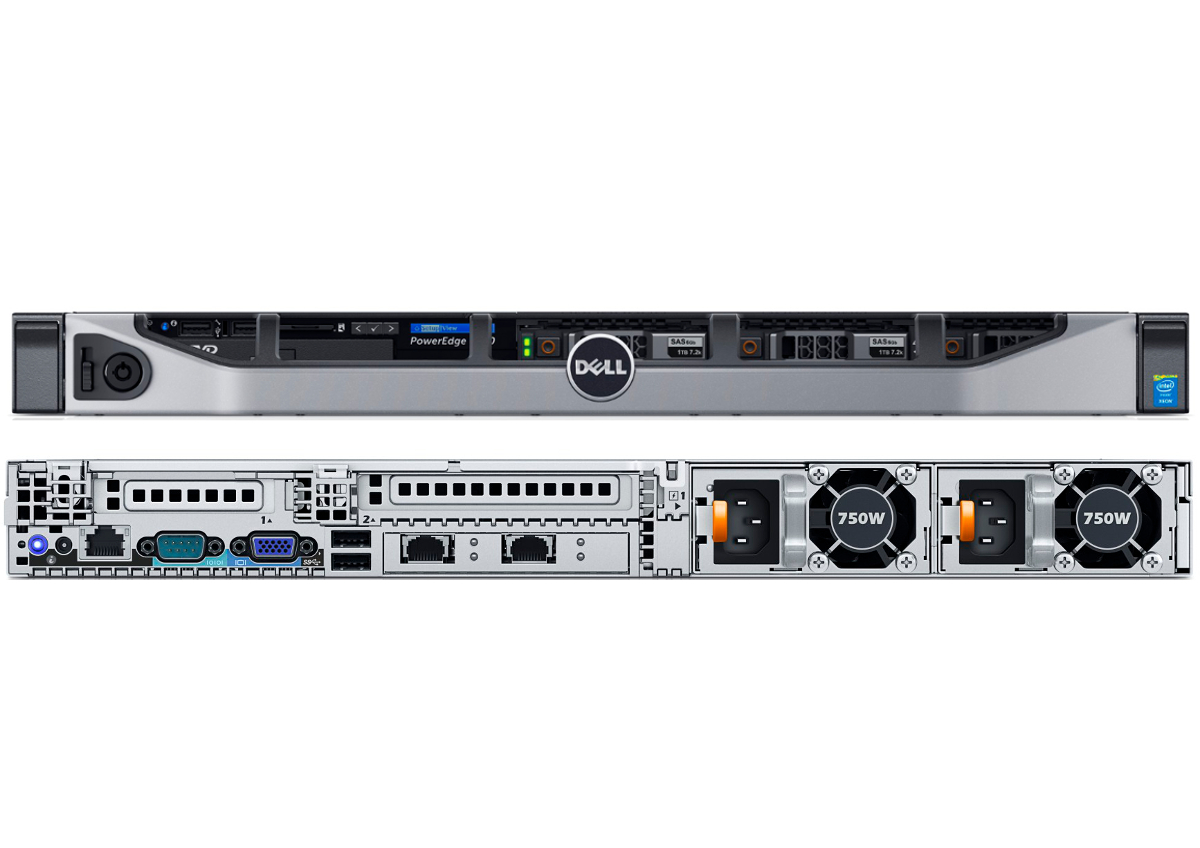
\includegraphics[width=\textwidth]{img/r630.jpg}
	\caption{Dell PowerEdge R630}
\end{figure}

Jest to wysoko wydajny serwer, który dzięki małych rozmiarów oszczędzi
miejsce w serwerowni oraz cechuje się niskim zużyciem
energii. Parametry techniczne serwera:

\begin{description}
\item[procesor] 2 sockety procesora (dla Intel® Xeon® E5 2600 v3)
\item[chipset] Intel C610
\item[pamięć RAM] do 768 GB (24 sloty DIMM) DDR4
\item[pamięć trwała] do 10 dysków (1,8 TB każdy)
\item[kontroler RAID] PERC H730P
\item[złącza I/O] do 3 złącz PCIe
\item[karta sieciowa] 4 x 1Gb, 2 x 1Gb + 2 x 10Gb, 4 x 10Gb
\item[obudowa] Rack 1U
\item[zasilanie] 2x 750W HotPlug
\end{description}

Aby serwer spełnił stawiane przed nim wymagania wydajnościowe należy
zakupić go w następującej konfiguracji:

\begin{description}
\item[procesor] 2x Intel® Xeon® Processor E5-2697 v3
\item[chipset] Intel C610
\item[pamięć RAM] 8x 16 GB DDR4
\item[pamięć trwała] 8x 146 GB 15k SAS (RAID 10)
\item[kontroler RAID] PERC H730P
\item[złącza I/O] do 3 złącz PCIe
\item[karta sieciowa] 4 x 1Gb, 2 x 1Gb + 2 x 10Gb, 4 x 10Gb
\item[obudowa] Rack 1U
\item[zasilanie] 2x 750W HotPlug
\end{description}

Zastosowanie dwóch serwerów o wskazanych parametrów pozwoli sprostać
wszystkim wymaganiom stawianym przez klienta. Ponadto zapewniona jest
możliwość skalowania dostarczonego rozwiązania poprzez dodanie
kolejnego serwera aplikacji lub rozbudowę (głównie pamięć operacyjna)
posiadanych już serwerów.

\subsubsection{Warstwa danych}

Serwer bazy danych powinien pozwalać na gromadzenie znacznej ilości
danych. Konieczne jest również zapewnienie redundantnego drugiego
serwera bazy danych, aby równoważyć obciążenie oraz zapewnić wysoką
dostępność. W celu zapewnienie odpowiednich możliwości w zakresie
przechowywania i przetwarzania dużej ilości danych postanowiono
wykożystać dwa serwery Dell PowerEdge R920.

\begin{figure}[H]
	\centering
	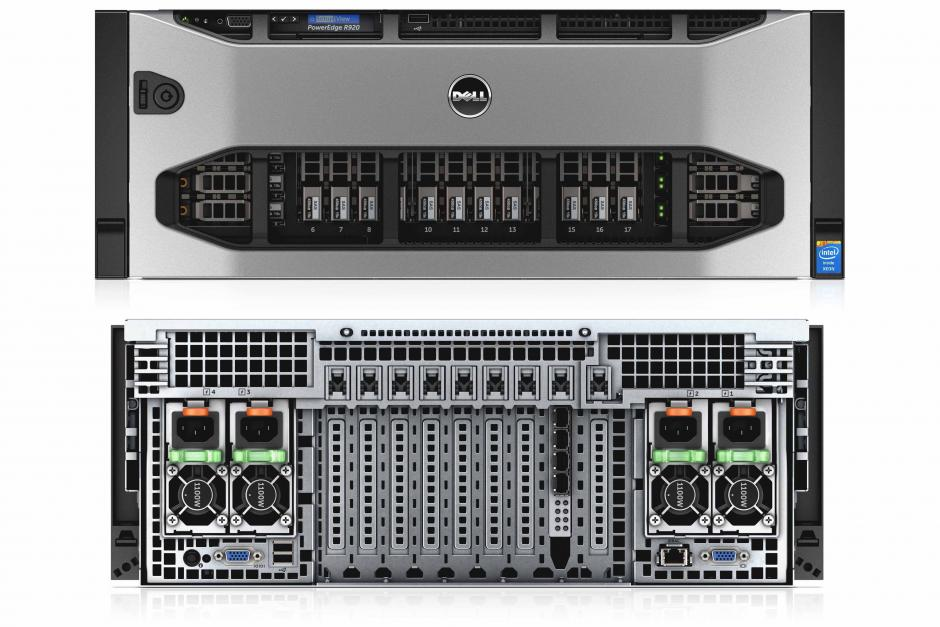
\includegraphics[width=\textwidth]{img/r920.jpg}
	\caption{Dell PowerEdge R920}
\end{figure}

Jest to wysokiej klasy serwer, którego parametry pozwolą na
przetwarzanie danych w czasie rzeczywistym. Parametry techniczne
serwera:

\begin{description}
\item[procesor] 4 sockety procesora (dla Intel Xeon E7-4800 v2 lub E7-8800 v2)
\item[chipset] Intel C602J
\item[pamięć RAM] do 6TB (96 slotów DIMM) DDR3L, RDIMM, LR-DIMM
\item[pamięć trwała] do 24 dysków (1,2 TB każdy)
\item[kontroler RAID] PERC H730P
\item[złącza I/O] do 10 złącz PCIe
\item[karta sieciowa] Intel Ethernet X540 10Gb BT DP + I350 1Gb BT DP
\item[karta graficzna] Matrox® G200 with 8MB memory
\item[obudowa] Rack 4U
\item[zasilanie] 4x 1100W HotPlug
\end{description}

Maksymalne parametry techniczne wybranego serwera znacząco
przewyższają bieżące zapotrzebowanie firmy dlatego wykorzystana
będzie następująca konfiguracja:

\begin{description}
\item[procesor] 2x Intel® Xeon® Processor E7-8880 v2 (37.5M Cache, 2.50 GHz)
\item[chipset] Intel C602J
\item[pamięć RAM] 8x 16 GB
\item[pamięć trwała] 2x 146 GB 15k SAS + 8x 1.2 TB
\item[kontroler RAID] PERC H730P
\item[złącza I/O] do 10 złącz PCIe
\item[karta sieciowa] Intel Ethernet X540 10Gb BT DP + I350 1Gb BT DP
\item[karta graficzna] Matrox® G200 with 8MB memory
\item[obudowa] Rack 4U
\item[zasilanie] 4x 1100W HotPlug
\end{description}

Zastosowana konfiguracja jest zdecydowanie wystarczająca dla
bieżących wymagań firmy, a zastosowanie wysokiej klasy serwera
pozostawia duże możliwości w zakresie skalowalności, dzięki czemu
serwery te będzie można dostosować do potrzeb intensywnie rozwijającej
się firmy. Dzięki wsparciu technologii wirtualizacji sprzętowej serwer
ten będzie mógł być efektywnie współdzielony z pozostałymi modułami
budowanego systemu.


\section{Specyfikacja przypadków użycia - poziom rozszerzony}
\newcommand{\myparagraph}[1]{\paragraph{#1}\mbox{}\\}

\subsection{Aktorzy}
\begin{itemize}
\item Użytkownik zasobów
\item Administrator zasobów
\item Serwisant
\item Menadżer
\end{itemize}


\subsection{PU1 Wyszukiwanie zasobów} \label{pu1}
\myparagraph{Opis}
Przypadek wyszukiwania zasobów za pomocą zadanych kryteriów przez użytkownika.

\myparagraph{Aktorzy}
Użytkownik zasobów.

\myparagraph{Warunki wstępne}
\begin{itemize}
\item Użytkownik jest zalogowany w systemie.
\end{itemize}

\myparagraph{Warunki końcowe}
Przypadek użycia nie wpływa na stan systemu.

\myparagraph{Przebieg podstawowy}
\begin{enumerate}
\item \label{pu1:f} Aktor wybiera ikonę wyszukiwania zasobów.
\item \label{pu1:s}System prezentuje okno wyszukiwania zasobów zawierające sekcję podawania kryteriów.
\item Aktor wprowadza kryteria wyszukiwania.
\item Aktor wciska przycisk ,,Wyszukaj''.
\item System prezentuje wyniki wyszukiwania.
\end{enumerate}

\myparagraph{Alternatywne przebiegi zdarzeń}
\begin{enumerate}
\item Aktor nie podał kryteriów wyszukiwania
	\begin{enumerate}[label*=\arabic*.]
	\item Kroki \ref{pu1:f} - \ref{pu1:s} jak w przebiegu podstawowym.
	\item Aktor wciska przycisk ,,Wyszukaj''.
	\item System wyświetla informację o konieczności podania kryteriów wyszukiwania.
	\end{enumerate}
\end{enumerate}

\myparagraph{Sytuacje wyjątkowe}
Brak połączenia z siecią.



\subsection{PU2 Obsługa sprzetu kopmuterowego} \label{pu2}
\subsubsection{PU2.1 Dodanie nowego sprzętu komputerowego do systemu}

\myparagraph{Opis}
Przypadek dodawania nowego sprzętu komputerowego do systemu katalogowego.

\myparagraph{Aktorzy}
Użytkownik zasobów.

\myparagraph{Warunki wstępne}
\begin{itemize}
\item Użytkownik jest zalogowany w systemie.
\end{itemize}

\myparagraph{Warunki końcowe}
\begin{itemize}
\item Do systemu katalogowego został dodany nowy sprzęt komputerowy.
\end{itemize}

\myparagraph{Przebieg podstawowy}
\begin{enumerate}
\item \label{pu2.1:1} Aktor wybiera ikonę dodawania sprzętu komputerowego.
\item System prezentuje okno dodawania sprzętu komputerowego.
\item Aktor podaje dane dodawanego zasobu.
\item \label{pu2.1:4} Aktor wciska przycisk ,,Dodaj''.
\item System wyświetla potwierdzenie dodania sprzętu komputerowego do systemu.
\end{enumerate}

\myparagraph{Alternatywne przebiegi zdarzeń}
\begin{enumerate}
\item Aktor nie posiada wystarczających uprawnień do dodania sprzętu komputerowego.
	\begin{enumerate}[label*=\arabic*.]
		\item Krok \ref{pu2.1:1} jak w przebiegu podstawowym.
		\item System wyświetla informację o brak wymaganych uprawnień.
	\end{enumerate}
\item Aktor podał niepoprawne lub niepełne dane sprzętu komputerowego.
	\begin{enumerate}[label*=\arabic*.]
		\item Kroki \ref{pu2.1:1} - \ref{pu2.1:4} jak w przebiegu podstawowym.
		\item System wyświetla informację o konieczności poprawienia danych.
	\end{enumerate}
\end{enumerate}

\myparagraph{Sytuacje wyjątkowe}
Brak połączenia z siecią.



\subsubsection{PU2.2 Edycja informacji o sprzęcie komputerowym}

\myparagraph{Opis}
Przypadek edycji danych sprzętu komputerowego znajdującego się w systemie katalogowym.

\myparagraph{Aktorzy}
Użytkownik zasobów.

\myparagraph{Warunki wstępne}
\begin{itemize}
\item Użytkownik jest zalogowany w systemie.
\item Sprzęt komputerowy istnieje w systemie katalogowym.
\end{itemize}

\myparagraph{Warunki końcowe}
\begin{itemize}
\item Dane sprzętu komputerowego zostały zmienione.
\end{itemize}

\myparagraph{Przebieg podstawowy}
\begin{enumerate}
\item \label{pu2.2:1} Aktor wyszukuje sprzęt zgodnie z \ref{pu1}
\item \label{pu2.2:2} Aktor wybiera sprzęt do edycji oraz wciska przycisk ,,Edytuj''.
\item System prezentuje okno edycji danych sprzętu komputerowego.
\item Aktor wprowadza nowe dane.
\item \label{pu2.2:5} Aktor wciska przycisk ,,Zapisz''.
\item System wyświetla potwierdzenie zmiany danych sprzętu komputerowego.
\end{enumerate}

\myparagraph{Alternatywne przebiegi zdarzeń}
\begin{enumerate}
\item Aktor nie posiada uprawnień do edycji danych sprzętu komputerowego.
	\begin{enumerate}[label*=\arabic*.]
		\item Kroki \ref{pu2.2:1} - \ref{pu2.2:2} jak w przebiegu podstawowym.
		\item System wyświetla informację o braku uprawnień do edycji.
	\end{enumerate}
\item Aktor podał niepoprawne lub niepełne dane sprzętu komputerowego.
	\begin{enumerate}[label*=\arabic*.]
		\item Kroki \ref{pu2.2:1} - \ref{pu2.2:5} jak w przebiegu podstawowym.
		\item System wyświetla informację o konieczności poprawienia danych.
	\end{enumerate}
\end{enumerate}

\myparagraph{Sytuacje wyjątkowe}\
Brak połączenia z siecią.

\subsubsection{PU2.3 Usunięcie sprzętu komputerowego z systemu}

\myparagraph{Opis}
Przypadek użycia opisuje procedurę usunięcia sprzętu komputerowego z systemu katalogowego.

\myparagraph{Aktorzy}
Użytkownik zasobów.

\myparagraph{Warunki wstępne}
\begin{itemize}
\item Użytkownik jest zalogowany w systemie.
\item Sprzęt komputerowy istnieje w systemie katalogowym.
\end{itemize}

\myparagraph{Warunki końcowe}
\begin{itemize}
\item Sprzęt komputerowy został usunięty z systemu katalogowego.
\end{itemize}

\myparagraph{Przebieg podstawowy}
\begin{enumerate}
\item \label{pu2.3:1} Aktor wyszukuje sprzęt zgodnie z \ref{pu1}
\item \label{pu2.3:2} Aktor wybiera sprzęt do usunięcia oraz wciska przycisk ,,Usuń''.
\item System wyświetla okno z prośbą o potwierdzenie wykonania operacji.
\item Aktor potwierdza wykonanie operacji.
\item System wyświetla potwierdzenie usunięcia sprzętu komputerowego z systemu.
\end{enumerate}

\myparagraph{Alternatywne przebiegi zdarzeń}
\begin{enumerate}
\item Aktor nie posiada uprawnień do usunięcia sprzętu komputerowego z systemu.
	\begin{enumerate}[label*=\arabic*.]
		\item Kroki \ref{pu2.3:1} - \ref{pu2.3:2} jak w przebiegu podstawowym.
		\item System wyświetla informację o braku uprawnień do usunięcia sprzętu komputerowego.
	\end{enumerate}
\end{enumerate}

\myparagraph{Sytuacje wyjątkowe}\
Brak połączenia z siecią.

\subsection{PU3 Obsługa oprogramowania} \label{pu3}
\subsubsection{PU3.1 Dodanie nowego oprogramowania}

\myparagraph{Opis}
Przypadek użycia opisuje procedurę dodania nowego oprogramowania do systemu katalogowego.

\myparagraph{Aktorzy}
Użytkownik zasobów.

\myparagraph{Warunki wstępne}
\begin{itemize}
\item Użytkownik jest zalogowany w systemie.
\end{itemize}

\myparagraph{Warunki końcowe}
\begin{itemize}
\item Oprogramowanie (wraz z danymi instalacji) zostało zapisane w systemie katalogowym.
\end{itemize}

\myparagraph{Przebieg podstawowy}
\begin{enumerate}
\item \label{pu3.1:1} Aktor wybiera ikonę dodawania oprogramowania.
\item System prezentuje okno dodawania oprogramowania.
\item Aktor podaje dane dodawanego zasobu wraz z informacjami na temat przeprowadzonych instalacji.
\item \label{pu3.1:4} Aktor wciska przycisk ,,Dodaj''.
\item System wyświetla potwierdzenie dodania oprogramowania do systemu katalogowego.
\end{enumerate}

\myparagraph{Alternatywne przebiegi zdarzeń}
\begin{enumerate}
\item Aktor nie posiada uprawnień do dodania oprogramowania.
	\begin{enumerate}[label*=\arabic*.]
		\item Krok \ref{pu3.1:1} jak w przebiegu podstawowym.
		\item System wyświetla informację o braku uprawnień do wykonania operacji dodania oprogramowania.
	\end{enumerate}
\item Aktor podał niepoprawne lub niepełne dane.
	\begin{enumerate}[label*=\arabic*.]
		\item Kroki \ref{pu3.1:1} - \ref{pu3.1:4} jak w przebiegu podstawowym.
		\item System wyświetla informację o konieczności poprawienia danych.
	\end{enumerate}
\end{enumerate}

\myparagraph{Sytuacje wyjątkowe}
Brak połączenia z siecią.

\subsubsection{PU3.2 Edycja informacji oprogramowaniu}

\myparagraph{Opis}
Przypadek użycia opisuje procedurę edycji informacji dotyczących oprogramowania znajdującego się w systemie - możliwa jest zmiana podstawowych danych oraz edycja przeprowadzonych instalacji.

\myparagraph{Aktorzy}
Użytkownik zasobów.

\myparagraph{Warunki wstępne}
\begin{itemize}
\item Użytkownik jest zalogowany w systemie.
\item Oprogramowanie istnieje w systemie katalogowym.
\end{itemize}

\myparagraph{Warunki końcowe}
\begin{itemize}
\item Dane oprogramowania zostały zmienione.
\end{itemize}

\myparagraph{Przebieg podstawowy}
\begin{enumerate}
\item \label{pu3.2:1} Aktor wyszukuje oprogramowanie zgodnie z \ref{pu1}
\item \label{pu3.2:2} Aktor wybiera oprogramowanie do edycji oraz wciska przycisk ,,Edytuj''.
\item System prezentuje okno edycji danych oprogramowania.
\item Aktor wprowadza nowe dane.
\item \label{pu3.2:5} Aktor wciska przycisk ,,Zapisz''.
\item System wyświetla potwierdzenie zmiany danych oprogramowania.
\end{enumerate}

\myparagraph{Alternatywne przebiegi zdarzeń}
\begin{enumerate}
\item Aktor nie posiada uprawnień do edycji danych oprogramowania.
	\begin{enumerate}[label*=\arabic*.]
		\item Kroki \ref{pu3.2:1} - \ref{pu3.2:2} jak w przebiegu podstawowym.
		\item System wyświetla informację o braku uprawnień do edycji.
	\end{enumerate}
\item Aktor podał niepoprawne lub niepełne dane oprogramowania.
	\begin{enumerate}[label*=\arabic*.]
		\item Kroki \ref{pu3.2:1} - \ref{pu3.2:5} jak w przebiegu podstawowym.
		\item System wyświetla informację o konieczności poprawienia danych.
	\end{enumerate}
\end{enumerate}

\myparagraph{Sytuacje wyjątkowe}\
Brak połączenia z siecią.

\subsubsection{PU3.3 Usunięcie oprogramowania z systemu}

\myparagraph{Opis}
Przypadek użycia opisuje procedurę usunięcia oprogramowania (wraz z danymi na temat przeprowadzonych instalacji) z systemu katalogowego.

\myparagraph{Aktorzy}
Użytkownik zasobów.

\myparagraph{Warunki wstępne}
\begin{itemize}
\item Użytkownik jest zalogowany w systemie.
\item Oprogramowanie istnieje w systemie katalogowym.
\end{itemize}

\myparagraph{Warunki końcowe}
\begin{itemize}
\item Oprogramowanie zostało usunięte z systemu katalogowego.
\end{itemize}

\myparagraph{Przebieg podstawowy}
\begin{enumerate}
\item \label{pu3.3:1} Aktor wyszukuje sprzęt zgodnie z \ref{pu1}
\item \label{pu3.3:2} Aktor wybiera oprogramowanie oraz wciska przycisk ,,Usuń''.
\item System wyświetla okno z prośbą o potwierdzenie wykonania operacji.
\item Aktor potwierdza wykonanie operacji.
\item System wyświetla potwierdzenie usunięcia oprogramowania z systemu.
\end{enumerate}

\myparagraph{Alternatywne przebiegi zdarzeń}
\begin{enumerate}
\item Aktor nie posiada uprawnień do usunięcia oprogramowania z systemu.
	\begin{enumerate}[label*=\arabic*.]
		\item Kroki \ref{pu3.3:1} - \ref{pu3.3:2} jak w przebiegu podstawowym.
		\item System wyświetla informację o braku uprawnień do usunięcia oprogramowania.
	\end{enumerate}
\end{enumerate}

\myparagraph{Sytuacje wyjątkowe}\
Brak połączenia z siecią.

\subsection{PU4 Obsługa innego sprzętu, urządzeń lub wyposażenia} \label{pu4}
\subsubsection{PU4.1 Dodanie innego sprzętu, urządzeń lub wyposażenia do systemu}

\myparagraph{Opis}
Przypadek użycia opisuje procedurę dodania sprzętu, urządzeń lub wyposażenia do systemu.

\myparagraph{Aktorzy}
Użytkownik zasobów.

\myparagraph{Warunki wstępne}
\begin{itemize}
\item Użytkownik jest zalogowany w systemie.
\end{itemize}

\myparagraph{Warunki końcowe}
\begin{itemize}
\item Zasób (wraz z danymi instalacji) został zapisany w systemie katalogowym.
\end{itemize}

\myparagraph{Przebieg podstawowy}
\begin{enumerate}
\item \label{pu4.1:1} Aktor wybiera ikonę dodawania zasobu.
\item System prezentuje okno dodawania zasobu.
\item Aktor podaje dane dodawanego zasobu.
\item \label{pu4.1:4} Aktor wciska przycisk ,,Dodaj''.
\item System wyświetla potwierdzenie dodania zasobu do systemu katalogowego.
\end{enumerate}

\myparagraph{Alternatywne przebiegi zdarzeń}
\begin{enumerate}
\item Aktor nie posiada uprawnień do dodania zasobu.
	\begin{enumerate}[label*=\arabic*.]
		\item Krok \ref{pu4.1:1} jak w przebiegu podstawowym.
		\item System wyświetla informację o braku uprawnień do wykonania operacji dodania zasobu.
	\end{enumerate}
\item Aktor podał niepoprawne lub niepełne dane.
	\begin{enumerate}[label*=\arabic*.]
		\item Kroki \ref{pu4.1:1} - \ref{pu4.1:4} jak w przebiegu podstawowym.
		\item System wyświetla informację o konieczności poprawienia danych.
	\end{enumerate}
\end{enumerate}

\myparagraph{Sytuacje wyjątkowe}
Brak połączenia z siecią.

\subsubsection{PU4.2 Edycja informacji o innym sprzęcie, urządzeniu lub wyposażeniu}

\myparagraph{Opis}
Przypadek użycia opisuje procedurę edycji informacji dotyczących ogólnych zasobów.

\myparagraph{Aktorzy}
Użytkownik zasobów.

\myparagraph{Warunki wstępne}
\begin{itemize}
\item Użytkownik jest zalogowany w systemie.
\item Zasób istnieje w systemie katalogowym.
\end{itemize}

\myparagraph{Warunki końcowe}
\begin{itemize}
\item Dane zasobu zostały zmienione.
\end{itemize}

\myparagraph{Przebieg podstawowy}
\begin{enumerate}
\item \label{pu4.2:1} Aktor wyszukuje zasób zgodnie z \ref{pu1}
\item \label{pu4.2:2} Aktor wybiera zasób do edycji oraz wciska przycisk ,,Edytuj''.
\item System prezentuje okno edycji danych zasobu.
\item Aktor wprowadza nowe dane.
\item \label{pu4.2:5} Aktor wciska przycisk ,,Zapisz''.
\item System wyświetla potwierdzenie zmiany danych zasobu.
\end{enumerate}

\myparagraph{Alternatywne przebiegi zdarzeń}
\begin{enumerate}
\item Aktor nie posiada uprawnień do edycji danych zasobu.
	\begin{enumerate}[label*=\arabic*.]
		\item Kroki \ref{pu4.2:1} - \ref{pu4.2:2} jak w przebiegu podstawowym.
		\item System wyświetla informację o braku uprawnień do edycji.
	\end{enumerate}
\item Aktor podał niepoprawne lub niepełne dane oprogramowania.
	\begin{enumerate}[label*=\arabic*.]
		\item Kroki \ref{pu4.2:1} - \ref{pu4.2:5} jak w przebiegu podstawowym.
		\item System wyświetla informację o konieczności poprawienia danych.
	\end{enumerate}
\end{enumerate}

\myparagraph{Sytuacje wyjątkowe}\
Brak połączenia z siecią.

\subsubsection{PU4.3 Usunięcie innego sprzętu, urządzenia lub wyposażenia z systemu}

\myparagraph{Opis}
Przypadek użycia opisuje procedurę usunięcia zasobu (ogólnego typu) z systemu katalogowego.

\myparagraph{Aktorzy}
Użytkownik zasobów.

\myparagraph{Warunki wstępne}
\begin{itemize}
\item Użytkownik jest zalogowany w systemie.
\item Zasób istnieje w systemie katalogowym.
\end{itemize}

\myparagraph{Warunki końcowe}
\begin{itemize}
\item Zasób został usunięty z systemu katalogowego.
\end{itemize}

\myparagraph{Przebieg podstawowy}
\begin{enumerate}
\item \label{pu4.3:1} Aktor wyszukuje zasób zgodnie z \ref{pu1}
\item \label{pu4.3:2} Aktor wybiera zasób oraz wciska przycisk ,,Usuń''.
\item System wyświetla okno z prośbą o potwierdzenie wykonania operacji.
\item Aktor potwierdza wykonanie operacji.
\item System wyświetla potwierdzenie usunięcia zasobu z systemu.
\end{enumerate}

\myparagraph{Alternatywne przebiegi zdarzeń}
\begin{enumerate}
\item Aktor nie posiada uprawnień do usunięcia zasobu z systemu.
	\begin{enumerate}[label*=\arabic*.]
		\item Kroki \ref{pu4.3:1} - \ref{pu4.3:2} jak w przebiegu podstawowym.
		\item System wyświetla informację o braku uprawnień do usunięcia zasobu.
	\end{enumerate}
\end{enumerate}

\myparagraph{Sytuacje wyjątkowe}\
Brak połączenia z siecią.

\subsection{PU5 Obsługa czasopisma lub zasobu literaturowego} \label{pu5}
\subsubsection{PU5.1 Dodanie nowego czasopisma lub zasobu literaturowego do systemu}

\myparagraph{Opis}
Przypadek użycia opisuje procedurę dodania czasopisma bądź zasobu literaturowego do systemu.

\myparagraph{Aktorzy}
Użytkownik zasobów.

\myparagraph{Warunki wstępne}
\begin{itemize}
\item Użytkownik jest zalogowany w systemie.
\end{itemize}

\myparagraph{Warunki końcowe}
\begin{itemize}
\item Dane czasopisma lub zasobu literackiego zostały zapisane w systemie katalogowym.
\end{itemize}

\myparagraph{Przebieg podstawowy}
\begin{enumerate}
\item \label{pu5.1:1} Aktor wybiera ikonę dodawania czasopisma/zasobu literaturowego.
\item System prezentuje okno dodawania zasobu.
\item Aktor podaje dane dodawanego zasobu.
\item \label{pu5.1:4} Aktor wciska przycisk ,,Dodaj''.
\item System wyświetla potwierdzenie dodania zasobu do systemu katalogowego.
\end{enumerate}

\myparagraph{Alternatywne przebiegi zdarzeń}
\begin{enumerate}
\item Aktor nie posiada uprawnień do dodania zasobu.
	\begin{enumerate}[label*=\arabic*.]
		\item Krok \ref{pu5.1:1} jak w przebiegu podstawowym.
		\item System wyświetla informację o braku uprawnień do wykonania operacji dodania zasobu.
	\end{enumerate}
\item Aktor podał niepoprawne lub niepełne dane.
	\begin{enumerate}[label*=\arabic*.]
		\item Kroki \ref{pu5.1:1} - \ref{pu5.1:4} jak w przebiegu podstawowym.
		\item System wyświetla informację o konieczności poprawienia danych.
	\end{enumerate}
\end{enumerate}

\myparagraph{Sytuacje wyjątkowe}
Brak połączenia z siecią.

\subsubsection{PU5.2 Edycja informacji o czasopiśmie lub zasobie literaturowym}

\myparagraph{Opis}
Przypadek użycia opisuje procedurę edycji informacji dotyczących czasopisma bądź zasobu literaturowego.

\myparagraph{Aktorzy}
Użytkownik zasobów.

\myparagraph{Warunki wstępne}
\begin{itemize}
\item Użytkownik jest zalogowany w systemie.
\item Czasopismo/zasób literaturowy istnieje w systemie katalogowym.
\end{itemize}

\myparagraph{Warunki końcowe}
\begin{itemize}
\item Dane zasobu zostały zmienione.
\end{itemize}

\myparagraph{Przebieg podstawowy}
\begin{enumerate}
\item \label{pu5.2:1} Aktor wyszukuje zasób zgodnie z \ref{pu1}
\item \label{pu5.2:2} Aktor wybiera zasób do edycji oraz wciska przycisk ,,Edytuj''.
\item System prezentuje okno edycji danych zasobu.
\item Aktor wprowadza nowe dane.
\item \label{pu5.2:5} Aktor wciska przycisk ,,Zapisz''.
\item System wyświetla potwierdzenie zmiany danych zasobu.
\end{enumerate}

\myparagraph{Alternatywne przebiegi zdarzeń}
\begin{enumerate}
\item Aktor nie posiada uprawnień do edycji danych zasobu.
	\begin{enumerate}[label*=\arabic*.]
		\item Kroki \ref{pu5.2:1} - \ref{pu5.2:2} jak w przebiegu podstawowym.
		\item System wyświetla informację o braku uprawnień do edycji.
	\end{enumerate}
\item Aktor podał niepoprawne lub niepełne dane oprogramowania.
	\begin{enumerate}[label*=\arabic*.]
		\item Kroki \ref{pu5.2:1} - \ref{pu5.2:5} jak w przebiegu podstawowym.
		\item System wyświetla informację o konieczności poprawienia danych.
	\end{enumerate}
\end{enumerate}

\myparagraph{Sytuacje wyjątkowe}\
Brak połączenia z siecią.

\subsubsection{PU5.3 Usunięcie czasopisma lub zasobu literaturowego z systemu}

\myparagraph{Opis}
Przypadek użycia opisuje procedurę usunięcia czasopisma/zasobu literaturowego z systemu katalogowego.

\myparagraph{Aktorzy}
Użytkownik zasobów.

\myparagraph{Warunki wstępne}
\begin{itemize}
\item Użytkownik jest zalogowany w systemie.
\item Czasopismo/zasób literaturowy istnieje w systemie katalogowym.
\end{itemize}

\myparagraph{Warunki końcowe}
\begin{itemize}
\item Czasopismo/zasób literaturowy został usunięty z systemu katalogowego.
\end{itemize}

\myparagraph{Przebieg podstawowy}
\begin{enumerate}
\item \label{pu5.3:1} Aktor wyszukuje zasób zgodnie z \ref{pu1}
\item \label{pu5.3:2} Aktor wybiera zasób oraz wciska przycisk ,,Usuń''.
\item System wyświetla okno z prośbą o potwierdzenie wykonania operacji.
\item Aktor potwierdza wykonanie operacji.
\item System wyświetla potwierdzenie usunięcia zasobu z systemu.
\end{enumerate}

\myparagraph{Alternatywne przebiegi zdarzeń}
\begin{enumerate}
\item Aktor nie posiada uprawnień do usunięcia zasobu z systemu.
	\begin{enumerate}[label*=\arabic*.]
		\item Kroki \ref{pu5.3:1} - \ref{pu5.3:2} jak w przebiegu podstawowym.
		\item System wyświetla informację o braku uprawnień do usunięcia zasobu.
	\end{enumerate}
\end{enumerate}

\myparagraph{Sytuacje wyjątkowe}\
Brak połączenia z siecią.


\subsection{PU6 Współpraca z modułem rejestru pracowników} \label{pu6}
\subsubsection{PU6.1 Zapisanie informacji o osobie odpowiedzialnej za zasób}
\myparagraph{Opis}
Przypadek zapisywania informacji o osobie, która odpowiada za zasób.

\myparagraph{Aktorzy}
Administrator zasobów.

\myparagraph{Warunki wstępne}
\begin{itemize}
\item Użytkownik jest zalogowany w systemie.
\item Osoba odpowiedzialna za zasób znajduje się w bazie pracowników.
\end{itemize}

\myparagraph{Warunki końcowe}
\begin{itemize}
\item Do systemu katalogowego została zapisana informacja o osobie odpowiedzialnej za zasób.
\end{itemize}

\myparagraph{Przebieg podstawowy}
\begin{enumerate}
	\item \label{pu6.1:1} Aktor wyszukuje zasób zgodnie z \ref{pu1}
	\item \label{pu6.1:2} Aktor wybiera sprzęt oraz wciska przycisk ,,Edytuj''.
	\item System prezentuje okno edycji zasobu.
	\item Aktor wybiera pracownika odpowiedzialnego za zasób ze zbioru wszystkich pracowników, mających uprawnienia do bycia odpowiedzialnym nad typem edytowanego zasobu.
	\item Aktor wciska przycisk „Zapisz”.
	\item System wyświetla potwierdzenie zmiany danych zasobu.
\end{enumerate}

\myparagraph{Alternatywne przebiegi zdarzeń}
\begin{enumerate}
	\item Aktor nie posiada uprawnień do edycji zasobu.
	\begin{enumerate}[label*=\arabic*.]
		\item Kroki \ref{pu6.1:1} - \ref{pu6.1:2} jak w przebiegu podstawowym.
		\item System wyświetla informację o braku uprawnień do edycji.
	\end{enumerate}
\end{enumerate}
\myparagraph{Sytuacje wyjątkowe}
Brak połączenia z siecią.

\subsubsection{PU6.2 Zapisanie informacji o użytkowniku konkretnego zasobu}
\myparagraph{Opis}
Przypadek zapisywania informacji o użytkownikach zasobu.

\myparagraph{Aktorzy}
Administrator zasobów.

\myparagraph{Warunki wstępne}
\begin{itemize}
\item Użytkownik jest zalogowany w systemie.
\item Osoba odpowiedzialna za zasób znajduje się w bazie pracowników.
\end{itemize}

\myparagraph{Warunki końcowe}
\begin{itemize}
\item Do systemu katalogowego została zapisana informacja o osobie użytkującej zasób.
\end{itemize}

\myparagraph{Przebieg podstawowy}
\begin{enumerate}
	\item \label{pu6.2:1} Aktor wyszukuje sprzęt zgodnie z \ref{pu1}
	\item \label{pu6.2:2} Aktor wybiera sprzęt oraz wciska przycisk ,,Edytuj''.
	\item System prezentuje okno edycji zasobu.
	\item Aktor modyfikuje listę użytkowników użytkujących dany zasób.
	\item Aktor wciska przycisk „Zapisz”.
	\item System wyświetla potwierdzenie zmiany danych zasobu.
\end{enumerate}

\myparagraph{Alternatywne przebiegi zdarzeń}
\begin{enumerate}
	\item Aktor nie posiada uprawnień do edycji zasobu.
	\begin{enumerate}[label*=\arabic*.]
		\item Kroki \ref{pu6.2:1} - \ref{pu6.2:2} jak w przebiegu podstawowym.
		\item System wyświetla informację o braku uprawnień do edycji.
	\end{enumerate}
\end{enumerate}

\myparagraph{Sytuacje wyjątkowe}
Brak połączenia z siecią.

\subsection{PU7 Obliczanie statystyk} \label{pu7}
\subsubsection{PU7.1 Prezentacja zakupów konkretnych zasobów w poszczególnych latach}
\myparagraph{Opis}
Przypadek prezentowania statystyk dotyczących ilości zakupów zasobów wybranych przez użytkownika w latach wybranych przez użytkownika.

\myparagraph{Aktorzy}
Menadżer.

\myparagraph{Warunki wstępne}
\begin{itemize}
\item Użytkownik jest zalogowany w systemie.
\end{itemize}

\myparagraph{Warunki końcowe}
\begin{itemize}
\item Użytkownik otrzymuje prezentacje statystyk dotyczących zakupów zasobów w latach.
\end{itemize}

\myparagraph{Przebieg podstawowy}
\begin{enumerate}
	\item \label{pu7.1:1} Aktor wybiera ikone generowania statystyk.
	\item System prezentuje dostępne typy raportów.
	\item \label{pu7.2:2} Aktor wybiera prezentacje statystyk dotyczących zakupów zasobów w latach.
	\item System prezentuje okno parametrów raportu.
	\item Aktor wybiera zasoby dla których mają być obliczane statystyki oraz wybiera lata dla których mają być wygenerowany raport.
	\item Aktor wciska przycisk „Generuj”.
	\item System wyświetla prezentacje statystyk.
\end{enumerate}

\myparagraph{Alternatywne przebiegi zdarzeń}
\begin{enumerate}
	\item Aktor nie posiada uprawnień generowania raportów.
	\begin{enumerate}[label*=\arabic*.]
		\item Krok \ref{pu6.1:1} jak w przebiegu podstawowym.
		\item System wyświetla informację o braku uprawnień do generowania raportów.
	\end{enumerate}
\end{enumerate}

\myparagraph{Sytuacje wyjątkowe}
Brak połączenia z siecią.

\subsubsection{PU7.2.1 Prezentacja ilości zakupionych zasobów w poszczególnych działach}
\myparagraph{Opis}
Przypadek prezentowania statystyk dotyczących ilości zakupów zasobów wybranych przez użytkownika w działach wybranych przez użytkownika.

\myparagraph{Aktorzy}
Menadżer.

\myparagraph{Warunki wstępne}
\begin{itemize}
\item Użytkownik jest zalogowany w systemie.
\end{itemize}

\myparagraph{Warunki końcowe}
\begin{itemize}
\item Użytkownik otrzymuje prezentacje statystyk dotyczących zakupów zasobów w działach.
\end{itemize}

\myparagraph{Przebieg podstawowy}
\begin{enumerate}
	\item \label{pu7.2.1:1} Aktor wybiera ikone generowania statystyk.
	\item System prezentuje dostępne typy raportów.
	\item \label{pu7.2.1:2} Aktor wybiera prezentacje statystyk dotyczących zakupów zasobów w działach.
	\item System prezentuje okno parametrów raportu.
	\item Aktor wybiera zasoby dla których mają być obliczane statystyki oraz wybiera działy dla których mają być wygenerowany raport.
	\item Aktor wciska przycisk „Generuj”.
	\item System wyświetla prezentacje statystyk.
\end{enumerate}

\myparagraph{Alternatywne przebiegi zdarzeń}
\begin{enumerate}
	\item Aktor nie posiada uprawnień generowania raportów.
	\begin{enumerate}[label*=\arabic*.]
		\item Krok \ref{pu6.1:1} jak w przebiegu podstawowym.
		\item System wyświetla informację o braku uprawnień do generowania raportów.
	\end{enumerate}
\end{enumerate}

\myparagraph{Sytuacje wyjątkowe}
Brak połączenia z siecią.

\subsubsection{PU7.2.2 Prezentacja ilości używanych zasobów w poszczególnych działach}
\myparagraph{Opis}
Przypadek prezentowania statystyk dotyczących ilości używanych zasobów wybranych przez użytkownika w działach wybranych przez użytkownika.

\myparagraph{Aktorzy}
Menadżer.

\myparagraph{Warunki wstępne}
\begin{itemize}
\item Użytkownik jest zalogowany w systemie.
\end{itemize}

\myparagraph{Warunki końcowe}
\begin{itemize}
\item Użytkownik otrzymuje prezentacje statystyk dotyczących użycia zasobów w działach.
\end{itemize}

\myparagraph{Przebieg podstawowy}
\begin{enumerate}
	\item \label{pu7.2.2:1} Aktor wybiera ikone generowania statystyk.
	\item System prezentuje dostępne typy raportów.
	\item \label{pu7.2.2:2} Aktor wybiera prezentacje statystyk dotyczących użycia zasobów w działach.
	\item System prezentuje okno parametrów raportu.
	\item Aktor wybiera zasoby dla których mają być obliczane statystyki oraz wybiera działy dla których mają być wygenerowany raport.
	\item Aktor wciska przycisk „Generuj”.
	\item System wyświetla prezentacje statystyk.
\end{enumerate}

\myparagraph{Alternatywne przebiegi zdarzeń}
\begin{enumerate}
	\item Aktor nie posiada uprawnień generowania raportów.
	\begin{enumerate}[label*=\arabic*.]
		\item Krok \ref{pu6.1:1} jak w przebiegu podstawowym.
		\item System wyświetla informację o braku uprawnień do generowania raportów.
	\end{enumerate}
\end{enumerate}

\myparagraph{Sytuacje wyjątkowe}
Brak połączenia z siecią.

\subsubsection{PU7.2.3 Prezentacja ilości napraw zasobów w poszczególnych działach}
\myparagraph{Opis}
Przypadek prezentowania statystyk dotyczących ilości napraw zasobów wybranych przez użytkownika w działach wybranych przez użytkownika.

\myparagraph{Aktorzy}
Menadżer.

\myparagraph{Warunki wstępne}
\begin{itemize}
\item Użytkownik jest zalogowany w systemie.
\end{itemize}

\myparagraph{Warunki końcowe}
\begin{itemize}
\item Użytkownik otrzymuje prezentacje statystyk dotyczących napraw zasobów w działach.
\end{itemize}

\myparagraph{Przebieg podstawowy}
\begin{enumerate}
	\item \label{pu7.2.3:1} Aktor wybiera ikone generowania statystyk.
	\item System prezentuje dostępne typy raportów.
	\item \label{pu7.2.3:2} Aktor wybiera prezentacje statystyk dotyczących napraw zasobów w działach.
	\item System prezentuje okno parametrów raportu.
	\item Aktor wybiera zasoby dla których mają być obliczane statystyki oraz wybiera działy dla których mają być wygenerowany raport.
	\item Aktor wciska przycisk „Generuj”.
	\item System wyświetla prezentacje statystyk.
\end{enumerate}

\myparagraph{Alternatywne przebiegi zdarzeń}
\begin{enumerate}
	\item Aktor nie posiada uprawnień generowania raportów.
	\begin{enumerate}[label*=\arabic*.]
		\item Krok \ref{pu6.1:1} jak w przebiegu podstawowym.
		\item System wyświetla informację o braku uprawnień do generowania raportów.
	\end{enumerate}
\end{enumerate}

\myparagraph{Sytuacje wyjątkowe}
Brak połączenia z siecią.

\subsubsection{PU7.3.1 Prezentacja ilości zakupionych zasobów w poszczególnych placówkach}
\myparagraph{Opis}
Przypadek prezentowania statystyk dotyczących ilości zakupów zasobów wybranych przez użytkownika w placówkach wybranych przez użytkownika.

\myparagraph{Aktorzy}
Menadżer.

\myparagraph{Warunki wstępne}
\begin{itemize}
\item Użytkownik jest zalogowany w systemie.
\end{itemize}

\myparagraph{Warunki końcowe}
\begin{itemize}
\item Użytkownik otrzymuje prezentacje statystyk dotyczących zakupu zasobów w placówkach.
\end{itemize}

\myparagraph{Przebieg podstawowy}
\begin{enumerate}
	\item \label{pu7.3.1:1} Aktor wybiera ikone generowania statystyk.
	\item System prezentuje dostępne typy raportów.
	\item \label{pu7.3.1:2} Aktor wybiera prezentacje statystyk dotyczących zakupów zasobów w placówkach.
	\item System prezentuje okno parametrów raportu.
	\item Aktor wybiera zasoby dla których mają być obliczane statystyki oraz wybiera placówki dla których mają być wygenerowany raport.
	\item Aktor wciska przycisk „Generuj”.
	\item System wyświetla prezentacje statystyk.
\end{enumerate}

\myparagraph{Alternatywne przebiegi zdarzeń}
\begin{enumerate}
	\item Aktor nie posiada uprawnień generowania raportów.
	\begin{enumerate}[label*=\arabic*.]
		\item Krok \ref{pu6.1:1} jak w przebiegu podstawowym.
		\item System wyświetla informację o braku uprawnień do generowania raportów.
	\end{enumerate}
\end{enumerate}

\myparagraph{Sytuacje wyjątkowe}
Brak połączenia z siecią.

\subsubsection{PU7.3.2 Prezentacja ilości używanych zasobów w poszczególnych placówkach}
\myparagraph{Opis}
Przypadek prezentowania statystyk dotyczących ilości używanych zasobów wybranych przez użytkownika w placówkach wybranych przez użytkownika.

\myparagraph{Aktorzy}
Menadżer.

\myparagraph{Warunki wstępne}
\begin{itemize}
\item Użytkownik jest zalogowany w systemie.
\end{itemize}

\myparagraph{Warunki końcowe}
\begin{itemize}
\item Użytkownik otrzymuje prezentacje statystyk dotyczących użycia zasobów w placówkach.
\end{itemize}

\myparagraph{Przebieg podstawowy}
\begin{enumerate}
	\item \label{pu7.3.2:1} Aktor wybiera ikone generowania statystyk.
	\item System prezentuje dostępne typy raportów.
	\item \label{pu7.3.2:2} Aktor wybiera prezentacje statystyk dotyczących użycia zasobów w placówkach.
	\item System prezentuje okno parametrów raportu.
	\item Aktor wybiera zasoby dla których mają być obliczane statystyki oraz wybiera placówki dla których mają być wygenerowany raport.
	\item Aktor wciska przycisk „Generuj”.
	\item System wyświetla prezentacje statystyk.
\end{enumerate}

\myparagraph{Alternatywne przebiegi zdarzeń}
\begin{enumerate}
	\item Aktor nie posiada uprawnień generowania raportów.
	\begin{enumerate}[label*=\arabic*.]
		\item Krok \ref{pu6.1:1} jak w przebiegu podstawowym.
		\item System wyświetla informację o braku uprawnień do generowania raportów.
	\end{enumerate}
\end{enumerate}

\myparagraph{Sytuacje wyjątkowe}
Brak połączenia z siecią.

\subsubsection{PU7.3.3 Prezentacja ilości napraw zasobów w poszczególnych placówkach}
\myparagraph{Opis}
Przypadek prezentowania statystyk dotyczących ilości napraw zasobów wybranych przez użytkownika w placówkach wybranych przez użytkownika.

\myparagraph{Aktorzy}
Menadżer.

\myparagraph{Warunki wstępne}
\begin{itemize}
\item Użytkownik jest zalogowany w systemie.
\end{itemize}

\myparagraph{Warunki końcowe}
\begin{itemize}
\item Użytkownik otrzymuje prezentacje statystyk dotyczących napraw zasobów w placówkach.
\end{itemize}

\myparagraph{Przebieg podstawowy}
\begin{enumerate}
	\item \label{pu7.3.3:1} Aktor wybiera ikone generowania statystyk.
	\item System prezentuje dostępne typy raportów.
	\item \label{pu7.3.3:2} Aktor wybiera prezentacje statystyk dotyczących napraw zasobów w placówkach.
	\item System prezentuje okno parametrów raportu.
	\item Aktor wybiera zasoby dla których mają być obliczane statystyki oraz wybiera działy dla których mają być wygenerowany raport.
	\item Aktor wciska przycisk „Generuj”.
	\item System wyświetla prezentacje statystyk.
\end{enumerate}

\myparagraph{Alternatywne przebiegi zdarzeń}
\begin{enumerate}
	\item Aktor nie posiada uprawnień generowania raportów.
	\begin{enumerate}[label*=\arabic*.]
		\item Krok \ref{pu6.1:1} jak w przebiegu podstawowym.
		\item System wyświetla informację o braku uprawnień do generowania raportów.
	\end{enumerate}
\end{enumerate}

\myparagraph{Sytuacje wyjątkowe}
Brak połączenia z siecią.

\subsection{PU8 Rejestracja informacji dotyczącej miejsca zakupu} \label{pu8}
\myparagraph{Opis}
Przypadek rejestracji miejsca zakupu zasobu.

\myparagraph{Aktorzy}
Administrator zasobów.

\myparagraph{Warunki wstępne}
\begin{itemize}
\item Użytkownik jest zalogowany w systemie.
\item Zasób jest już wprowadzony do bazy systemu.
\end{itemize}

\myparagraph{Warunki końcowe}
\begin{itemize}
\item Do systemu katalogowego została zapisana informacja dotycząca miejsca zakupu zasobu.
\end{itemize}

\myparagraph{Przebieg podstawowy}
\begin{enumerate}
	\item \label{pu8:1} Aktor wyszukuje zasób zgodnie z \ref{pu1}
	\item \label{pu8:2} Aktor wybiera zasób oraz wciska przycisk ,,Edytuj''.
	\item System prezentuje okno edycji zasobu.
	\item Aktor wprowadza informacje dotyczącą miejsca zakupu zasobu.
	\item Aktor wciska przycisk „Zapisz”.
	\item System wyświetla potwierdzenie zmiany danych zasobu.
\end{enumerate}

\myparagraph{Alternatywne przebiegi zdarzeń}
\begin{enumerate}
	\item Aktor nie posiada uprawnień do edycji zasobu.
	\begin{enumerate}[label*=\arabic*.]
		\item Kroki \ref{pu8:1} - \ref{pu8:2} jak w przebiegu podstawowym.
		\item System wyświetla informację o braku uprawnień do edycji.
	\end{enumerate}
\end{enumerate}

\myparagraph{Sytuacje wyjątkowe}
Brak połączenia z siecią.

\subsection{PU9 Historia napraw sprzętu} \label{pu9}
\subsubsection{PU9.1 Rejestracja informacji o wewnętrznej naprawie sprzętu}
\myparagraph{Opis}
Przypadek rejestracji informacji naprawie sprzętu dokonanej wewnątrz firmy.

\myparagraph{Aktorzy}
Serwisant.

\myparagraph{Warunki wstępne}
\begin{itemize}
\item Użytkownik jest zalogowany w systemie.
\item Sprzęt jest już wprowadzony do bazy systemu.
\end{itemize}

\myparagraph{Warunki końcowe}
\begin{itemize}
\item Do systemu katalogowego została zapisana informacja dotycząca wewnętrznej naprawy sprzętu.
\end{itemize}

\myparagraph{Przebieg podstawowy}
\begin{enumerate}
	\item \label{pu9.1:1} Aktor wyszukuje sprzęt zgodnie z \ref{pu1}
	\item \label{pu9.1:2} Aktor wybiera sprzęt oraz wciska przycisk ,,Edytuj''.
	\item System prezentuje okno edycji sprzętu.
	\item \label{pu9.1:4} Aktor wprowadza informacje o przeprowadzonej wewnętrznej naprawie sprzętu.
	\item Aktor wciska przycisk „Zapisz”.
	\item System wyświetla potwierdzenie zmiany danych sprzętu.
\end{enumerate}

\myparagraph{Alternatywne przebiegi zdarzeń}
\begin{enumerate}
	\item Aktor nie posiada uprawnień do edycji sprzętu.
	\begin{enumerate}[label*=\arabic*.]
		\item Kroki \ref{pu9.1:1} - \ref{pu9.1:2} jak w przebiegu podstawowym.
		\item System wyświetla informację o braku uprawnień do edycji.
	\end{enumerate}
	\item Niepoprawny okres przebywania w naprawie.
	\begin{enumerate}[label*=\arabic*.]
		\item Kroki \ref{pu9.1:1} - \ref{pu9.1:4} jak w przebiegu podstawowym.
		\item System wyświetla informację o nakładaniu się okresów naprawy z innym wpisem o naprawie.
	\end{enumerate}
\end{enumerate}

\myparagraph{Sytuacje wyjątkowe}
Brak połączenia z siecią.

\subsubsection{PU9.2 Rejestracja informacji o zewnętrznej naprawie sprzętu}
\myparagraph{Opis}
Przypadek rejestracji informacji naprawie sprzętu dokonanej w firmie zewnętrznej.

\myparagraph{Aktorzy}
Serwisant.

\myparagraph{Warunki wstępne}
\begin{itemize}
\item Użytkownik jest zalogowany w systemie.
\item Sprzęt jest już wprowadzony do bazy systemu.
\end{itemize}

\myparagraph{Warunki końcowe}
\begin{itemize}
\item Do systemu katalogowego została zapisana informacja dotycząca zewnętrznej naprawy sprzętu.
\end{itemize}

\myparagraph{Przebieg podstawowy}
\begin{enumerate}
	\item \label{pu9.2:1} Aktor wyszukuje sprzęt zgodnie z \ref{pu1}
	\item \label{pu9.2:2} Aktor wybiera sprzęt oraz wciska przycisk ,,Edytuj''.
	\item System prezentuje okno edycji sprzętu.
	\item \label{pu9.2:4} Aktor wprowadza informacje o przeprowadzonej zewnętrznej naprawie sprzętu.
	\item Aktor wciska przycisk „Zapisz”.
	\item System wyświetla potwierdzenie zmiany danych sprzętu.
\end{enumerate}

\myparagraph{Alternatywne przebiegi zdarzeń}
\begin{enumerate}
	\item Aktor nie posiada uprawnień do edycji sprzętu.
	\begin{enumerate}[label*=\arabic*.]
		\item Kroki \ref{pu9.2:1} - \ref{pu9.2:2} jak w przebiegu podstawowym.
		\item System wyświetla informację o braku uprawnień do edycji.
	\end{enumerate}
	\item Niepoprawny okres przebywania w naprawie.
	\begin{enumerate}[label*=\arabic*.]
		\item Kroki \ref{pu9.2:1} - \ref{pu9.2:4} jak w przebiegu podstawowym.
		\item System wyświetla informację o nakładaniu się okresów naprawy z innym wpisem o naprawie.
	\end{enumerate}
\end{enumerate}

\myparagraph{Sytuacje wyjątkowe}
Brak połączenia z siecią.

\subsection{PU10 Rejestracja aktualizacji oprogramowania} \label{pu10}
\myparagraph{Opis}
Przypadek rejestracji instalacji aktualizacji oprogramowania.

\myparagraph{Aktorzy}
Serwisant.

\myparagraph{Warunki wstępne}
\begin{itemize}
\item Użytkownik jest zalogowany w systemie.
\item Oprogramowanie jest już wprowadzone do bazy systemu.
\end{itemize}

\myparagraph{Warunki końcowe}
\begin{itemize}
\item Do systemu katalogowego została zapisana informacja dotycząca instalacji aktualizacji oprogramowania.
\end{itemize}

\myparagraph{Przebieg podstawowy}
\begin{enumerate}
	\item \label{pu10:1} Aktor wyszukuje oprogramowanie zgodnie z \ref{pu1}
	\item \label{pu10:2} Aktor wybiera oprogramowanie oraz wciska przycisk ,,Edytuj''.
	\item System prezentuje okno edycji oprogramowania.
	\item \label{pu10:4} Aktor wprowadza informacje o przeprowadzonej instalacji aktualizacji oprogramowania.
	\item Aktor wciska przycisk „Zapisz”.
	\item System wyświetla potwierdzenie zmiany danych oprogramowania.
\end{enumerate}

\myparagraph{Alternatywne przebiegi zdarzeń}
\begin{enumerate}
	\item Aktor nie posiada uprawnień do edycji oprogramowania.
	\begin{enumerate}[label*=\arabic*.]
		\item Kroki \ref{pu10:1} - \ref{pu10:2} jak w przebiegu podstawowym.
		\item System wyświetla informację o braku uprawnień do edycji.
	\end{enumerate}
	\item Aktualizacja oprogramowania została już przeprowadzona.
	\begin{enumerate}[label*=\arabic*.]
		\item Kroki \ref{pu10:1} - \ref{pu10:4} jak w przebiegu podstawowym.
		\item System wyświetla informację o tym, że wprowadzana aktualizacja została już przeprowadzona.
	\end{enumerate}
\end{enumerate}

\myparagraph{Sytuacje wyjątkowe}
Brak połączenia z siecią.

\subsection{PU11 Rejestracja operacji serwisowej} \label{pu11}
\myparagraph{Opis}
Przypadek rejestracji faktu serwisowania sprzętu.

\myparagraph{Aktorzy}
Serwisant.

\myparagraph{Warunki wstępne}
\begin{itemize}
\item Serwisant zalogowany w systemie.
\item Sprzęt jest już wprowadzony do bazy systemu.
\end{itemize}

\myparagraph{Warunki końcowe}
\begin{itemize}
\item Do systemu katalogowego została zapisana informacja dotycząca przeprowadzonej operacji serwisowej.
\end{itemize}

\myparagraph{Przebieg podstawowy}
\begin{enumerate}
	\item \label{pu11:1} Aktor wyszukuje sprzęt zgodnie z \ref{pu1}
	\item \label{pu11:2} Aktor wybiera sprzęt oraz wciska przycisk ,,Edytuj''.
	\item System prezentuje okno edycji sprzęt.
	\item Aktor wprowadza informacje o przeprowadzonej operacji serwisowej.
	\item Aktor wciska przycisk „Zapisz”.
	\item System wyświetla potwierdzenie zmiany danych sprzętu.
\end{enumerate}

\myparagraph{Alternatywne przebiegi zdarzeń}
\begin{enumerate}
	\item Aktor nie posiada uprawnień do edycji sprzętu.
	\begin{enumerate}[label*=\arabic*.]
		\item Kroki \ref{pu11:1} - \ref{pu11:2} jak w przebiegu podstawowym.
		\item System wyświetla informację o braku uprawnień do edycji.
	\end{enumerate}
\end{enumerate}


\myparagraph{Sytuacje wyjątkowe}
Brak połączenia z siecią.
\section{Analityczny model projektowy dziedziny}
\subsection{Diagram klas}
\begin{figure}[h!]
	\centering
	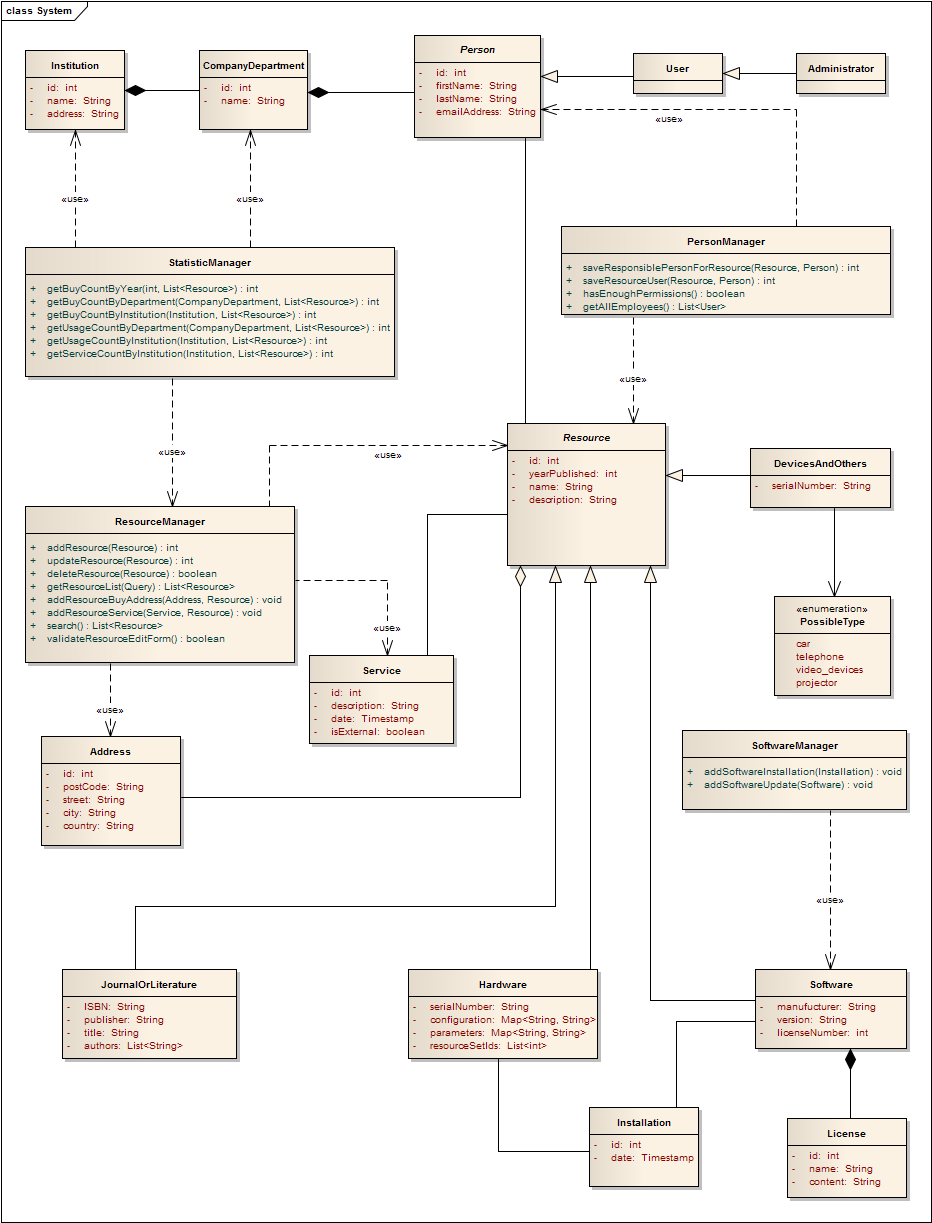
\includegraphics[scale=0.4]{img/class-diagram2}
	\caption{Diagram klas systemu.\label{fig:labelClassDiagram}}
\end{figure}

\newpage 

Opis klas przedstawionych na diagramie~\ref{fig:labelClassDiagram}:
\begin{description}
	\item \textbf{\textit{Person}} - klasa abstrakcyjna, będąca bazową dla klas \textit{User} oraz \textit{Administrator}. Przechowuje podstawowe informacje o osobie zawierające identyfikator, imię, nazwisko oraz adres email.
	
	\item \textbf{User} - specjalizacja klasy abstrakcyjnej \textit{Person} będąca użytkownikiem zasobu przechowywanego przez system.
	
	\item \textbf{Administrator} - specjalizacja klasy \textit{User} nadająca dodatkowe cechy polegające na umożliwieniu administrowania zasobami w systemie.
	
	\item \textbf{CompanyDepartment} - klasa słownikowa reprezentująca dział firmy. Komponuje osoby firmy.
	
	\item \textbf{Institution} - klasa reprezentująca oddział firmy. Komponuje działy firmy.
	
	\item \textbf{\textit{Resource}} - klasa abstrakcyjna reprezentująca byt w systemie. Jest generalizacją takich typów jak \textit{Software}, \textit{Hardware}, \textit{JournalOrLiterature} oraz \textit{DevicesAndOthers}. Zawiera informacje o identyfikatorze, roku produkcji, nazwa oraz opis.
	
	\item \textbf{Software} - klasa reprezentująca oprogramowanie. Jest specjalizacją klasy \textit{Resource}. Składa się z takich atrybutów jak wytwórca, wersja oraz numer licencji.
	
	\item \textbf{Hardware} - klasa reprezentująca sprzęt komputerowy. Jest specjalizacją klasy \textit{Resource}. Zawiera takie informacje jak numer seryjny, konfigurację, parametry oraz potencjalne zestawy w skład których może wchodzić.
		
	\item \textbf{JournalOrLiterature} - klasa reprezentująca czasopisma oraz literaturę. Jest specjalizacją klasy \textit{Resource}. W skład jej atrybutów wchodzą numer ISBN, wydawca, autor oraz tytuł.
		
	\item \textbf{DevicesAndOthers} - klasa reprezentująca inny sprzęt taki jak samochody, telefony itp (zdefiniowane w enumeracji \textit{PossibleType}). Jest specjalizacją klasy \textit{Resource}. Jej atrybutem jest numer seryjny.
	
	\item \textbf{PossibleType} - enumeracja definiujące możliwe typy innych urządzeń. Są nimi samochody, telefony, sprzęt video oraz projektory.
	
	\item \textbf{License} - klasa reprezentująca byt licencji wchodząca w skład obiektu \textit{Software}.
	
	\item \textbf{Installation} - klasa asocjacyjna łącząca obiekty \textit{Software} oraz \textit{Hardware}.
	
	\item \textbf{Service} - klasa reprezentująca usługę serwisową. W skład jej atrybutów wchodzą identyfikator, opis, data wykonania oraz flaga mówiąca o tym czy usługa serwisowa była wykonana wewnątrz firmy czy została zlecona zewnętrznie.
	
	\item \textbf{Address} - klasa reprezentująca obiekt adresu. Składa się z identyfikatora, kodu pocztowego, ulicy, miasta oraz kraju. Jest agregowana przez obiekt \textit{Resource}.
	
	\item \textbf{PersonManager} - klasa zarządzająca obiektami \textit{Person} oraz \textit{Resource}. Umożliwia wykonanie operacji zapisu użytkownika zasobu jak również osoby odpowiedzialnej za zasób.
	
	\item \textbf{ResourceManager} - klasa zarządzająca obiektami \textit{Resource}, \textit{Service} oraz \textit{Address}. Umożliwia wykonywanie operacji dodania, aktualizacji, usunięcia zasobu. Dodatkowo umożliwia pobieranie zasobów wedle zadanego zapytania oraz dodanie adresu zasobu oraz usługi serwisowej danego zasobu. 
		
	\item \textbf{SoftwareManager} - klasa zarządzająca obiektami \textit{Software}. Umożliwia na dodanie informacji o instalacji oraz aktualizacji zasobu.
			
	\item \textbf{StatisticManager} - klasa korzystająca z obiektów \textit{Institution}, \textit{CompanyDepartment} oraz wykorzystująca zarządce zasobów - \textit{ResouceManager}. Umożliwia na uzyskanie statystyk zakupu zasobów w poszczególnych latach, z uwzględnieniem działu oraz instytucji. Ponadto umożliwia uzyskanie informacji o użyciu zasobu w dziale firmy, instytucji oraz liczbie wykonanych usług serwisowych w instytucji.
\end{description}

\newpage
\subsection{Diagramy sekwencji}
Przykładowe diagramy sekwencji wykorzystujące obiekty pokazane na diagramie klas.
\begin{figure}[h!]
	\centering
	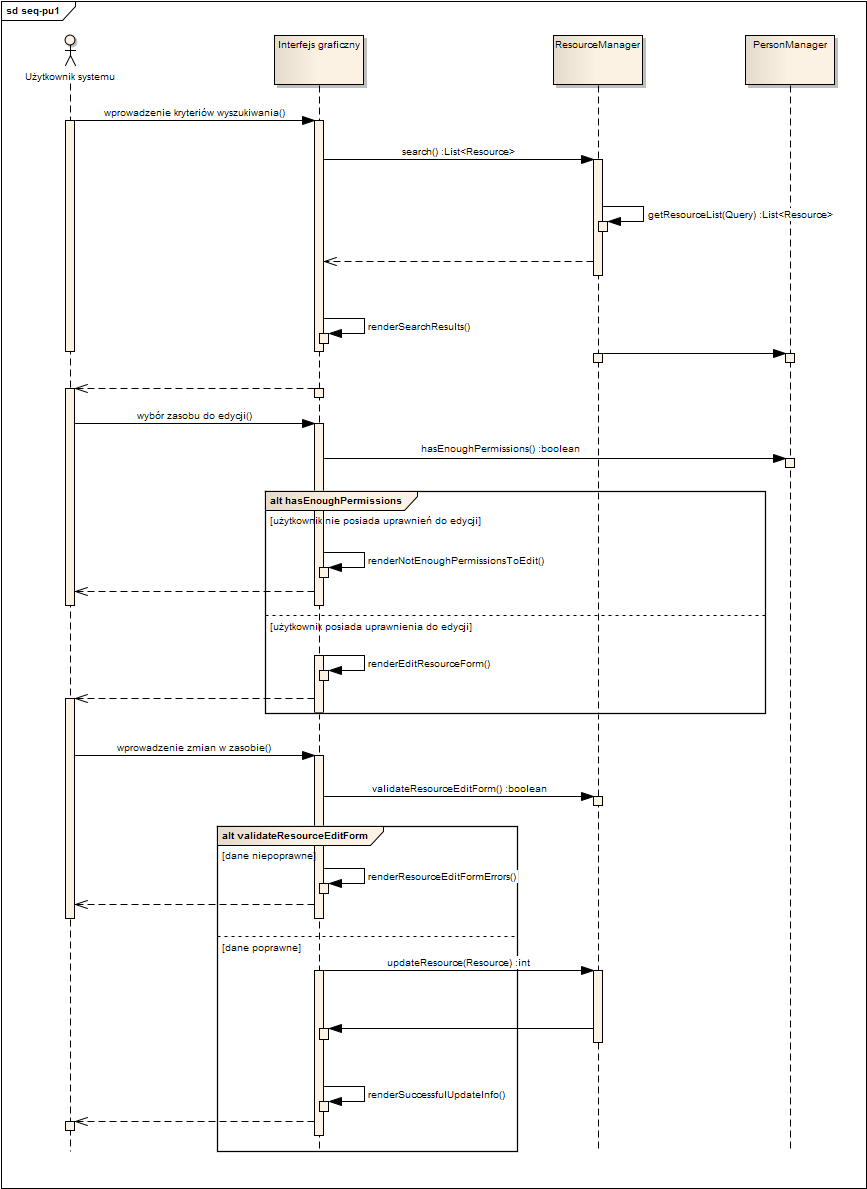
\includegraphics[scale=0.4]{img/seq-pu-a}
	\caption{Edycja danych zasobu.\label{fig:seq-pu-a}}
\end{figure}
\begin{figure}[h!]
	\centering
	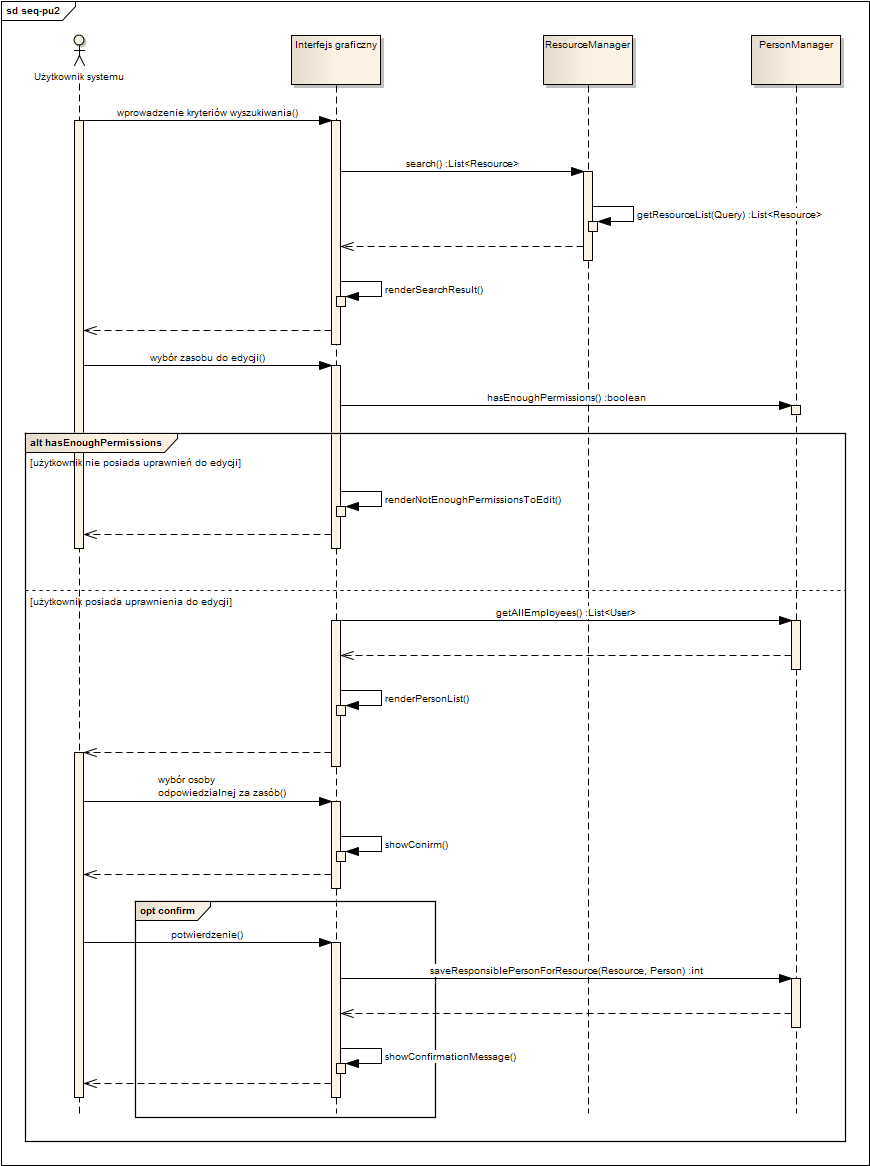
\includegraphics[scale=0.4]{img/seq-pu-b}
	\caption{Przypisanie osoby odpowiedzialnej za zasób.\label{fig:seq-pu-b}}
\end{figure}
\section{Logiczny model danych}

\begin{figure}[h!]
	\centering
	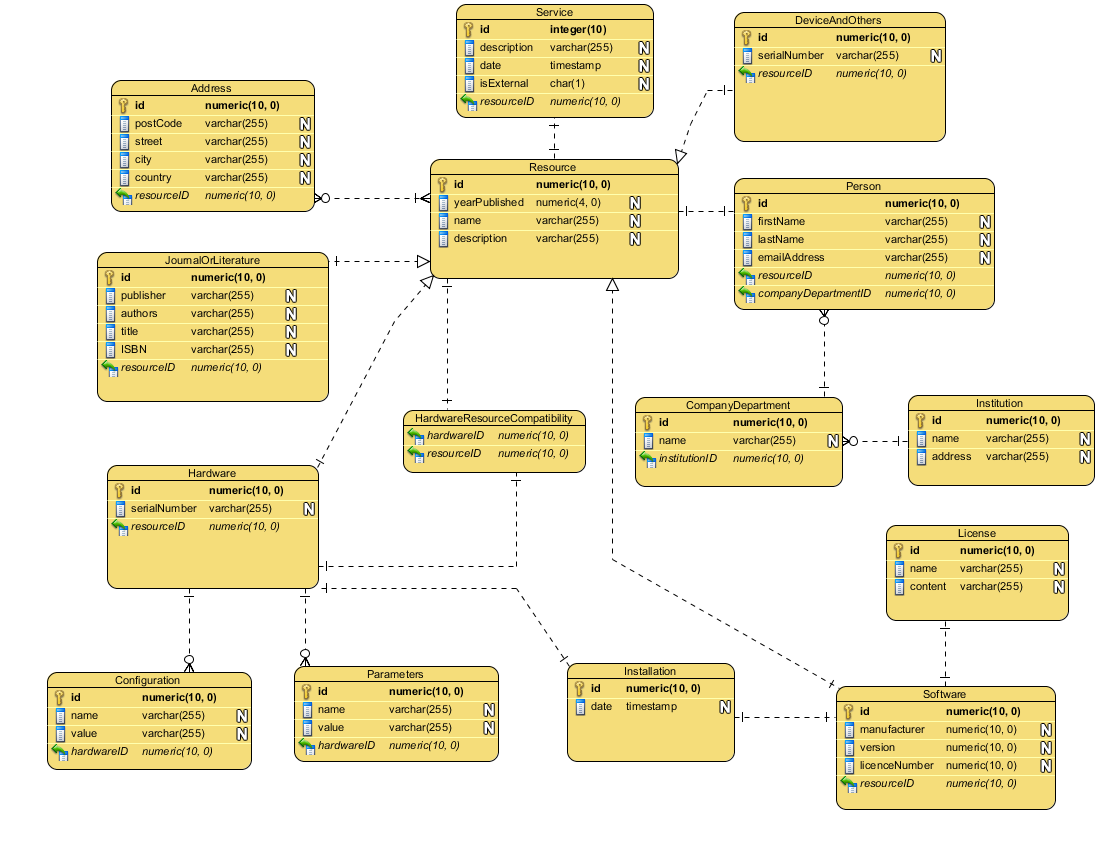
\includegraphics[scale=0.57, angle=270]{img/diagrams/LDM/LDM}
	\caption{Logiczny model danych\label{fig:labelLDM}}
\end{figure}
\bigskip
\subsection{Opis tabel}

\subsubsection{Address}
Odpowiada za przechowywanie adresu zasobu.
\begin{table}[H]
	\renewcommand\arraystretch{1.5}
	\renewcommand\tabcolsep{1.5pt}
\begin{tabular}{| c | c | c | c |} 
	\hline \textbf{Nazwa atrybutu} & \textbf{Znaczenie atrybutu} & \textbf{Typ danych} & \textbf{Ograniczenia} \\ 
	\hline ID & PRIMARY KEY & Numeric(10,0) & NOT NULL, UNIQUE \\ 
	\hline postCode & Kod pocztowy & Varchar(255) & REGEXP LIKE \\
	~ & ~ & ~ & \verb|[([0-9]\{2}-[0-9]\{3})| \\ 
	\hline street & Ulica & Varchar(255) &  \\ 
	\hline city & Miasto & Varchar(255) & \\ 
	\hline country & Kraj & Varchar(255) &  \\ 
	\hline resourceID & FOREIGN KEY & Numeric(10,0) & \\ 
	\hline 
\end{tabular}
\caption{Tabela Address}
\label{TAB:Address}
\end{table} 

\subsubsection{Service}
Przechowuje usługę serwisową.
\begin{table}[H]
	\renewcommand\arraystretch{1.5}
	\renewcommand\tabcolsep{1pt}
	\begin{tabular}{| c | c | c | c |} 
	\hline \textbf{Nazwa atrybutu} & \textbf{Znaczenie atrybutu} & \textbf{Typ danych} & \textbf{Ograniczenia} \\ 
	\hline ID & PRIMARY KEY & Numeric(10,0) & NOT NULL, UNIQUE \\ 
	\hline Description & Opis & Varchar(255) & \\ 
	\hline Date & Data & Timestamp &  \\ 
	\hline isExternal & Czy usługa została zlecona zewnętrznie? & Char(1) & \\ 
	\hline resourceID & FOREIGN KEY & Numeric(10,0) & \\ 
	\hline 
\end{tabular}
\caption{Tabela Service}
\label{TAB:Service}
\end{table} 

\subsubsection{Person}
Reprezentuje osobę (użytkownik, administrator).
\begin{table}[H]
	\renewcommand\arraystretch{1.5}
	\renewcommand\tabcolsep{3pt}
\begin{tabular}{| c | c | c | c |}
	\hline \textbf{Nazwa atrybutu} & \textbf{Znaczenie atrybutu} & \textbf{Typ danych} & \textbf{Ograniczenia} \\ 
	\hline ID & PRIMARY KEY & Numeric(10,0) & NOT NULL, UNIQUE \\ 
	\hline firstName & Imię & Varchar(255) & \\ 
	\hline lastName & Nazwisko & Varchar(255) &  \\ 
	\hline emailAddress & Adres email & Varchar(255) & REGEXP LIKE\\
	~ & ~ & ~ & \verb|[a-z0-9_.-]|\\ 
	~ & ~ & ~ & \verb|+@[a-z0-9_.-]|\\ 
	~ & ~ & ~ & \verb|+\.\ w {2,4}|\\ 
	\hline resourceID & FOREIGN KEY & Numeric(10,0) & \\ 
	\hline companyDepartmentID & FOREIGN KEY & Numeric(10,0) & \\ 
	\hline 
\end{tabular} 
\caption{Tabela Person}
\label{TAB:Person}
\end{table}

\subsubsection{CompanyDepartment}
Reprezentuje dział firmy.
\begin{table}[H]
	\renewcommand\arraystretch{1.5}
	\renewcommand\tabcolsep{3pt}
	\begin{tabular}{| c | c | c | c |} 
		\hline \textbf{Nazwa atrybutu} & \textbf{Znaczenie atrybutu} & \textbf{Typ danych} & \textbf{Ograniczenia} \\ 
		\hline ID & PRIMARY KEY & Numeric(10,0) & NOT NULL, UNIQUE \\ 
		\hline Name & Nazwa działu & Varchar(255) &  \\ 
		\hline institutionID & FOREIGN KEY & Numeric(10,0) & \\ 
		\hline 
	\end{tabular} 
	\caption{Tabela CompanyDepartment}
	\label{TAB:CompanyDepartment}
\end{table}

\subsubsection{Institution}
Reprezentuje oddział firmy.
\begin{table}[H]
	\renewcommand\arraystretch{1.5}
	\renewcommand\tabcolsep{3pt}
	\begin{tabular}{| c | c | c | c |} 
		\hline \textbf{Nazwa atrybutu} & \textbf{Znaczenie atrybutu} & \textbf{Typ danych} & \textbf{Ograniczenia} \\ 
		\hline ID & PRIMARY KEY & Numeric(10,0) & NOT NULL, UNIQUE \\ 
		\hline Name & Nazwa oddziału & Varchar(255) &  \\ 
		\hline Address & Adres & Varchar(255) & \\ 
		\hline 
	\end{tabular} 
	\caption{Tabela Institution}
	\label{TAB:Institution}
\end{table}

\subsubsection{License}
Reprezentuje licencję.
\begin{table}[H]
	\renewcommand\arraystretch{1.5}
	\renewcommand\tabcolsep{3pt}
	\begin{tabular}{| c | c | c | c |} 
		\hline \textbf{Nazwa atrybutu} & \textbf{Znaczenie atrybutu} & \textbf{Typ danych} & \textbf{Ograniczenia} \\ 
		\hline ID & PRIMARY KEY & Numeric(10,0) & NOT NULL, UNIQUE \\ 
		\hline Name & Nazwa & Varchar(255) &  \\ 
		\hline Content & Zawartość & Varchar(255) & \\ 
		\hline 
	\end{tabular} 
	\caption{Tabela License}
	\label{TAB:License}
\end{table}

\subsubsection{Installation}
Reprezentuje instalację (powiązanie software z hardware).
\begin{table}[H]
	\renewcommand\arraystretch{1.5}
	\renewcommand\tabcolsep{3pt}
	\begin{tabular}{| c | c | c | c |} 
		\hline \textbf{Nazwa atrybutu} & \textbf{Znaczenie atrybutu} & \textbf{Typ danych} & \textbf{Ograniczenia} \\ 
		\hline ID & PRIMARY KEY & Numeric(10,0) & NOT NULL, UNIQUE \\ 
		\hline Date & Data instalacji & timestamp &  \\ 
		\hline 
	\end{tabular} 
	\caption{Tabela Installation}
	\label{TAB:Installation}
\end{table}

\subsubsection{Configuration}
Reprezentuje konfigurację.
\begin{table}[H]
	\renewcommand\arraystretch{1.5}
	\renewcommand\tabcolsep{3pt}
	\begin{tabular}{| c | c | c | c |} 
		\hline \textbf{Nazwa atrybutu} & \textbf{Znaczenie atrybutu} & \textbf{Typ danych} & \textbf{Ograniczenia} \\ 
		\hline ID & PRIMARY KEY & Numeric(10,0) & NOT NULL, UNIQUE \\ 
		\hline Name & Nazwa konfigurowanej wartości & Varchar(255) &  \\ 
		\hline Name & Wartość & Varchar(255) &  \\
		\hline hardwareID & FOREIGN KEY & Numeric(10,0) & \\ 
		\hline 
	\end{tabular} 
	\caption{Tabela Configuration}
	\label{TAB:Configuration}
\end{table}

\subsubsection{Parameters}
Reprezentuje parametry (parametry i ich wartości).
\begin{table}[H]
	\renewcommand\arraystretch{1.5}
	\renewcommand\tabcolsep{3pt}
	\begin{tabular}{| c | c | c | c |} 
		\hline \textbf{Nazwa atrybutu} & \textbf{Znaczenie atrybutu} & \textbf{Typ danych} & \textbf{Ograniczenia} \\ 
		\hline ID & PRIMARY KEY & Numeric(10,0) & NOT NULL, UNIQUE \\ 
		\hline Name & Nazwa parametru & Varchar(255) &  \\ 
		\hline Name & Wartość & Varchar(255) &  \\
		\hline hardwareID & FOREIGN KEY & Numeric(10,0) & \\ 
		\hline 
	\end{tabular} 
	\caption{Tabela Parameters}
	\label{TAB:Parameters}
\end{table}

\subsubsection{Resource}
Reprezentuje zasób w firmie. Tabela jest podstawą do rozszerzania.
\begin{table}[H]
	\renewcommand\arraystretch{1.5}
	\renewcommand\tabcolsep{3pt}
	\begin{tabular}{| c | c | c | c |} 
		\hline \textbf{Nazwa atrybutu} & \textbf{Znaczenie atrybutu} & \textbf{Typ danych} & \textbf{Ograniczenia} \\ 
		\hline ID & PRIMARY KEY & numeric(10,0) & NOT NULL, UNIQUE \\ 
		\hline name & Nazwa zasobu & varchar(255) & NOT NULL  \\
		\hline description & Opis zasobu & varchar(255) & \\ 
		\hline 
	\end{tabular} 
	\caption{Tabela Resource}
	\label{TAB:Resource}
\end{table}

\subsubsection{JournalOrLiterature}
Reprezentuje czasopismo lub zasób książkowy. Rozszerza tabelę Resources.
\begin{table}[H]
	\renewcommand\arraystretch{1.5}
	\renewcommand\tabcolsep{3pt}
	\begin{tabular}{| c | c | c | c |} 
		\hline \textbf{Nazwa atrybutu} & \textbf{Znaczenie atrybutu} & \textbf{Typ danych} & \textbf{Ograniczenia} \\ 
		\hline ID & PRIMARY KEY & numeric(10,0) & NOT NULL, UNIQUE \\ 
		\hline publisher & Wydawca & varchar(255) & NOT NULL \\ 
		\hline yearPublished & Data publikacji & numeric(4,0) & \\
		\hline authors & Autorzy & varchar(255) & NOT NULL \\
		\hline title & Tytuł & varchar(255) & NOT NULL \\ 
		\hline ISBN & ISBN & varchar(255) & NOT NULL \\ 
		\hline resourceID & FOREIGN KEY & numeric(10,0) & NOT NULL \\ 
		\hline 
	\end{tabular} 
	\caption{Tabela Resource}
	\label{TAB:Resource}
\end{table}

\subsubsection{Hardware}
Reprezentuje zasób sprzętowy. Rozszerza tabelę Resources.
\begin{table}[H]
	\renewcommand\arraystretch{1.5}
	\renewcommand\tabcolsep{3pt}
	\begin{tabular}{| c | c | c | c |} 
		\hline \textbf{Nazwa atrybutu} & \textbf{Znaczenie atrybutu} & \textbf{Typ danych} & \textbf{Ograniczenia} \\ 
		\hline ID & PRIMARY KEY & numeric(10,0) & NOT NULL, UNIQUE \\ 
		\hline serialNumber & Numer seryjny & varchar(255) & NOT NULL \\ 
		\hline resourceID & FOREIGN KEY & numeric(10,0) & NOT NULL \\ 
		\hline 
	\end{tabular} 
	\caption{Tabela Hardware}
	\label{TAB:Hardware}
\end{table}

\subsubsection{HardwareResourceCompatibility}
Reprezentuje kompatybilność sprzętu z zasobami.
\begin{table}[H]
	\renewcommand\arraystretch{1.5}
	\renewcommand\tabcolsep{3pt}
	\begin{tabular}{| c | c | c | c |} 
		\hline \textbf{Nazwa atrybutu} & \textbf{Znaczenie atrybutu} & \textbf{Typ danych} & \textbf{Ograniczenia} \\ 
		\hline ID & PRIMARY KEY & numeric(10,0) & NOT NULL, UNIQUE \\ 
		\hline hardwareId & Numer seryjny & numeric(10,0) & NOT NULL \\ 
		\hline resourceID & FOREIGN KEY & numeric(10,0) & NOT NULL \\ 
		\hline 
	\end{tabular} 
	\caption{Tabela HardwareResourceCompatibility}
	\label{TAB:HardwareResourceCompatibility}
\end{table}

\subsubsection{DeviceAndOthers}
Reprezentuje urządzenia oraz inne zasoby. Rozszerza tabelę Resources.
\begin{table}[H]
	\renewcommand\arraystretch{1.5}
	\renewcommand\tabcolsep{3pt}
	\begin{tabular}{| c | c | c | c |} 
		\hline \textbf{Nazwa atrybutu} & \textbf{Znaczenie atrybutu} & \textbf{Typ danych} & \textbf{Ograniczenia} \\ 
		\hline ID & PRIMARY KEY & numeric(10,0) & NOT NULL, UNIQUE \\ 
		\hline serialNumber & Numer seryjny & varchar(255) & NOT NULL \\ 
		\hline resourceID & FOREIGN KEY & numeric(10,0) & NOT NULL \\ 
		\hline 
	\end{tabular} 
	\caption{Tabela DeviceAndOthers}
	\label{TAB:DeviceAndOthers}
\end{table}

\subsubsection{Software}
Reprezentuje oprogramowanie. Rozszerza tabelę Resources.
\begin{table}[H]
	\renewcommand\arraystretch{1.5}
	\renewcommand\tabcolsep{3pt}
	\begin{tabular}{| c | c | c | c |} 
		\hline \textbf{Nazwa atrybutu} & \textbf{Znaczenie atrybutu} & \textbf{Typ danych} & \textbf{Ograniczenia} \\ 
		\hline ID & PRIMARY KEY & numeric(10,0) & NOT NULL, UNIQUE \\ 
		\hline manufacturer & Wytwórca & numeric(10,0) & NOT NULL \\ 
		\hline version & Wersja & numeric(10,0) & NOT NULL \\ 
		\hline licenceNumber & Numer licencji & numeric(10,0) & NOT NULL \\ 
		\hline resourceID & FOREIGN KEY & numeric(10,0) & NOT NULL \\ 
		\hline 
	\end{tabular} 
	\caption{Tabela Software}
	\label{TAB:Software}
\end{table}
\section{Projekt interfejsu użytkownika}
\subsection{Logowanie}

\begin{figure}[H]
	\centering
        \vfill
        \noindent
        \makebox[\textwidth]{
          
\includegraphics[width=1.2\textwidth]{img/screens/logowanie.png}
        }
	\caption{Ekran logowania}
\end{figure}

\subsection{Wyszukiwanie zasobu}

\begin{figure}[H]
	\centering
        \vfill
        \noindent
        \makebox[\textwidth]{
          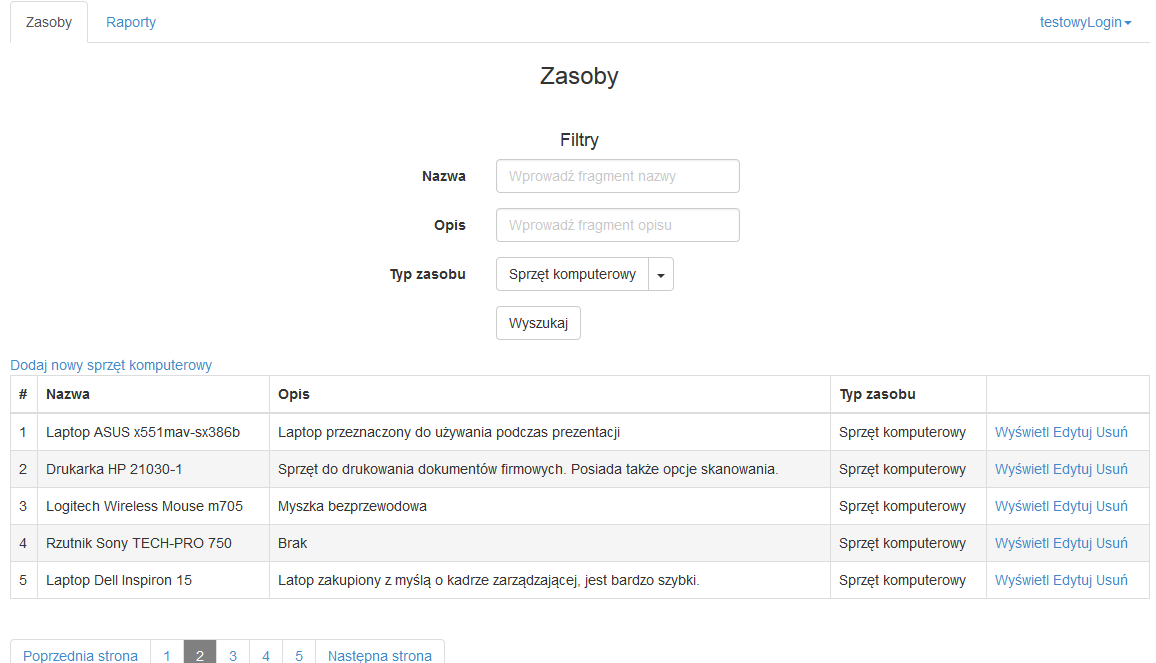
\includegraphics[width=1.2\textwidth]{img/screens/wyszZasob.png}
        }
	\caption{Ekran wyszukiwania zasobów}
\end{figure}

\subsection{Dodawanie sprzętu komputerowego}
\begin{figure}[H]
	\centering
        \vfill
        \noindent
        \makebox[\textwidth]{
          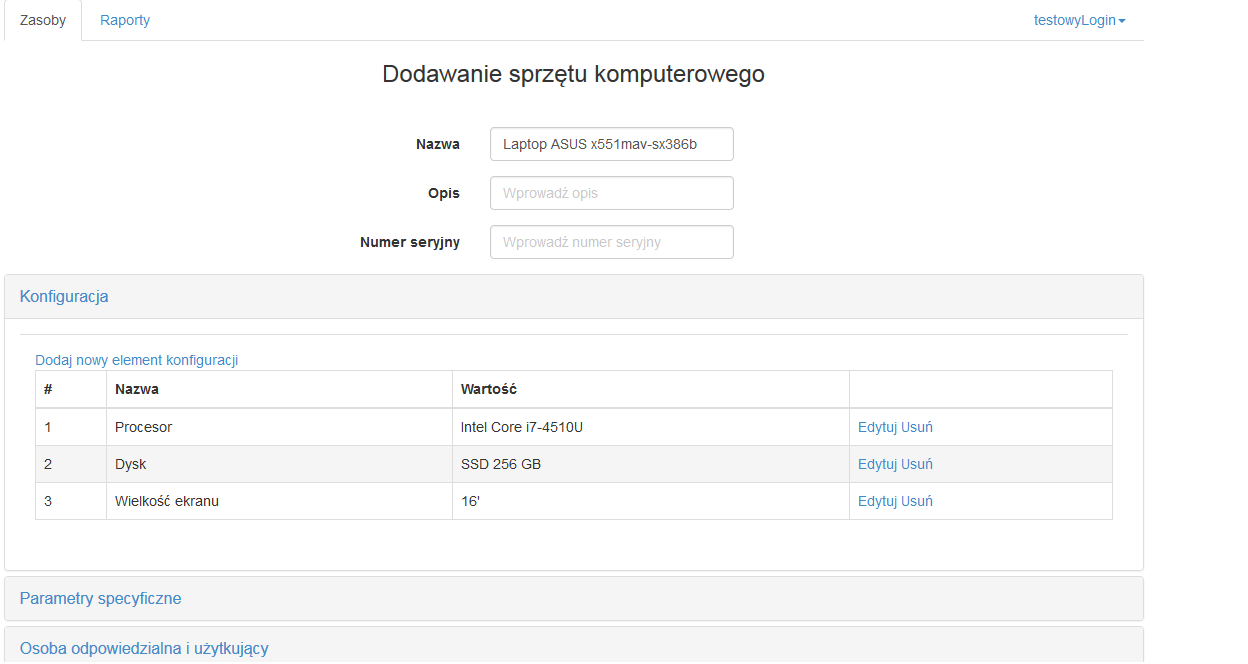
\includegraphics[width=1.2\textwidth]{img/screens/dodawanieSprzetuKomputerowego.png}
        }
	\caption{Ekran dodawania sprzętu komputerowego}
\end{figure}

\subsection{Zapisanie informacji o użytkowniku oprogramowania}
\begin{figure}[H]
	\centering
        \vfill
        \noindent
        \makebox[\textwidth]{
          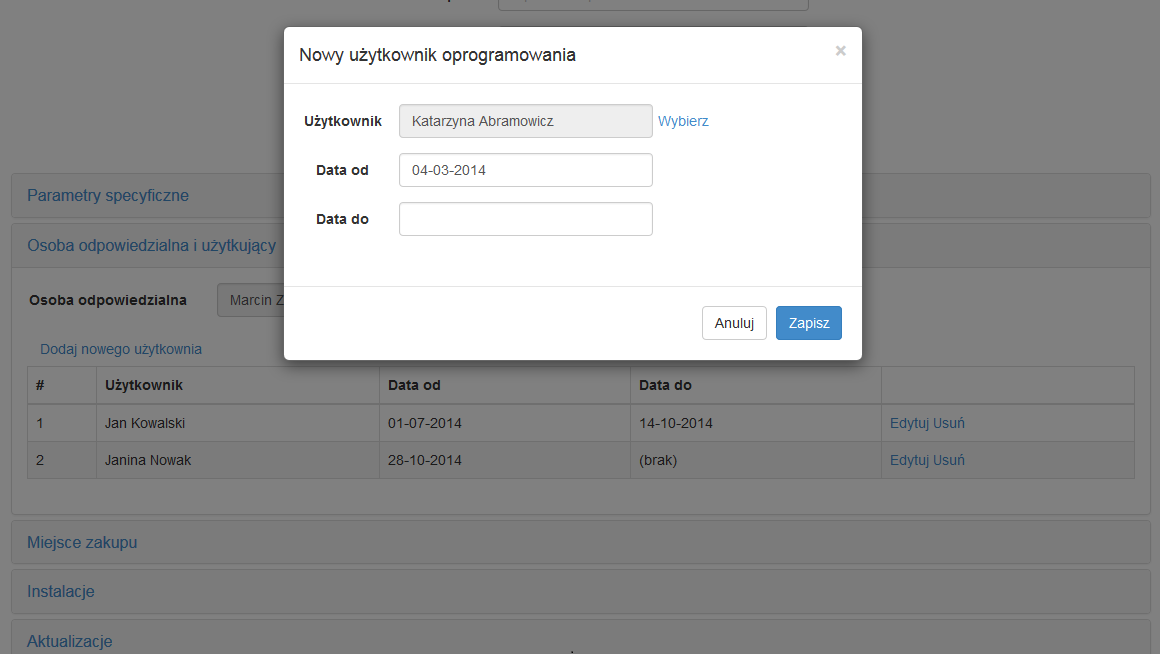
\includegraphics[width=1.2\textwidth]{img/screens/nowyUzytkownikOprogramowania.png}
        }
	\caption{Dodawanie użytkownika oprogramowania}
\end{figure}

\subsection{Rejestracja miejsca zakupu literatury lub zasobu literaturowego}
\begin{figure}[H]
	\centering
        \vfill
        \noindent
        \makebox[\textwidth]{
          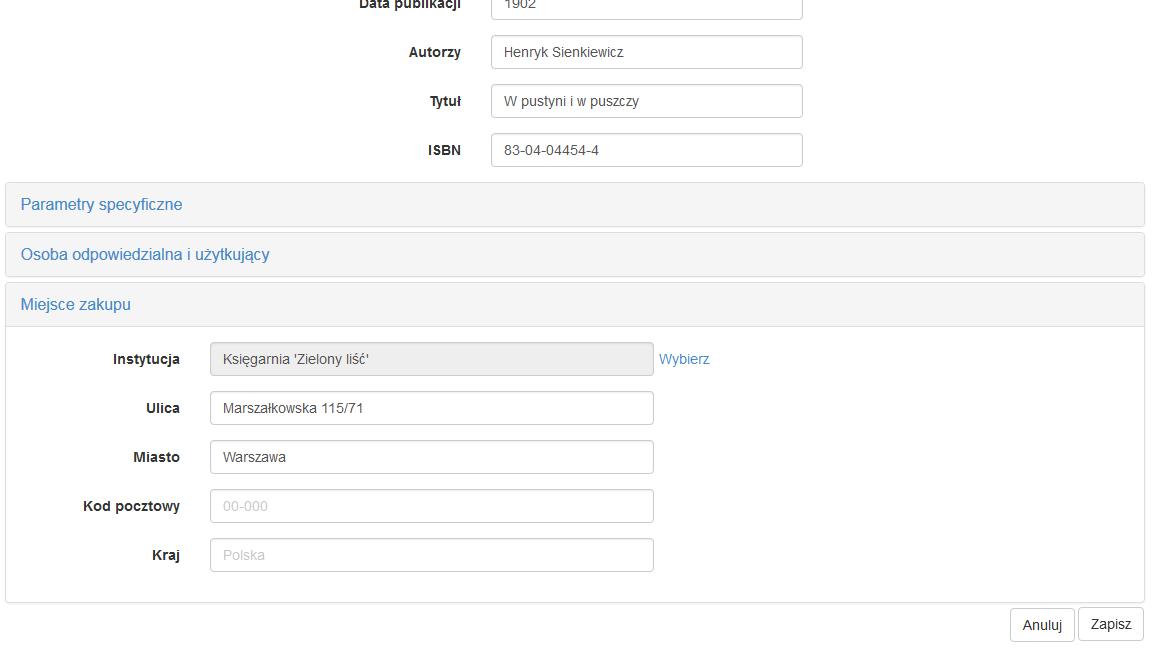
\includegraphics[width=1.2\textwidth]{img/screens/miejsceZakupuLiteratura.png}
        }
	\caption{Edycja informacji na temat miejsca zakupu}
\end{figure}

\subsection{Edytowanie historii napraw sprzędu}
\begin{figure}[H]
	\centering
        \vfill
        \noindent
        \makebox[\textwidth]{
          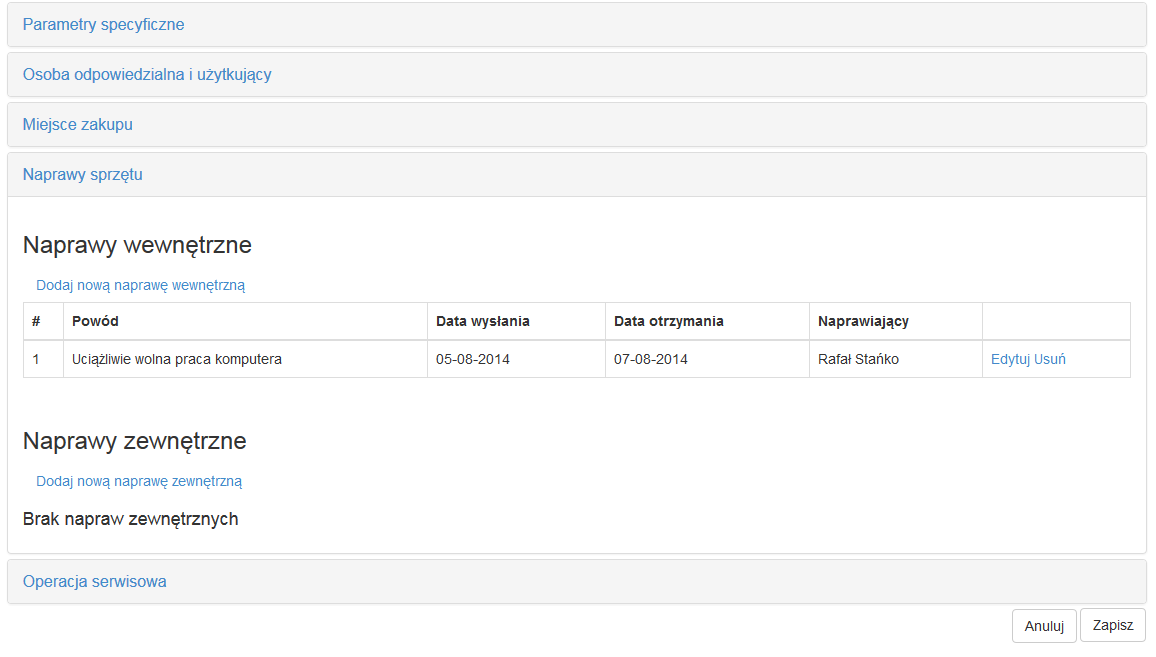
\includegraphics[width=1.2\textwidth]{img/screens/naprawyWew.png}
        }
	\caption{Modyfikacja historii napraw sprzętu}
\end{figure}

\subsection{Prezentacja ilosci zakupionych zasobow w dzialach}
\begin{figure}[H]
	\centering
        \vfill
        \noindent
        \makebox[\textwidth]{
          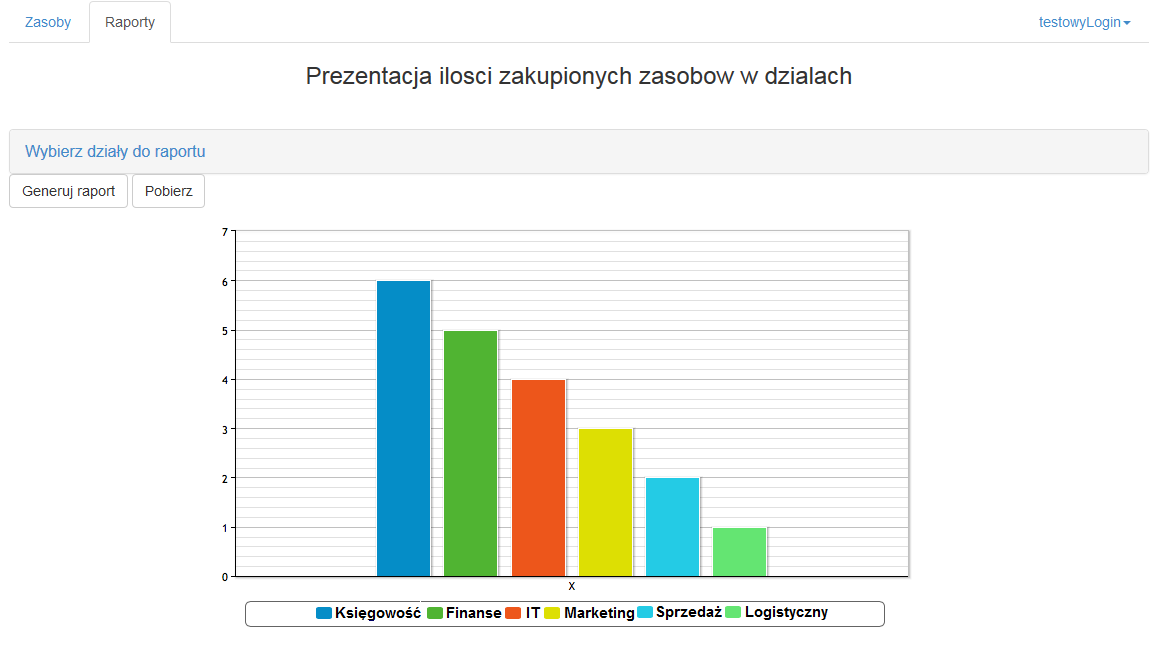
\includegraphics[width=1.2\textwidth]{img/screens/raport.png}
        }
	\caption{Przykładowy raport - prezentacja ilosci zakupionych zasobow w dzialach}
\end{figure}


\end{document}

% % % % % szablon do wstawiania obrazków
%\begin{figure}[h!]
%	\centering
%	\includegraphics[scale=0.5]{sciezka-do-pliku}
%	\caption{podpis \label{fig:label1}}
%\end{figure}